\documentclass[10pt,twocolumn,letterpaper]{article}

% ============================================================================
% Standard Packages (100% compatible with TeX Live & Overleaf out of the box)
% ============================================================================
\usepackage[utf8]{inputenc}
\usepackage[T1]{fontenc}
\usepackage{lmodern}
\usepackage{microtype}
\usepackage[margin=0.72in,columnsep=0.24in]{geometry}

\usepackage{amsmath,amssymb,amsfonts,amsthm,mathtools}
\usepackage{booktabs}
\usepackage{multirow}
\usepackage{tabularx}
\usepackage{array}
\usepackage{graphicx}
\usepackage{xcolor}
\usepackage{listings}
\usepackage{enumitem}
\usepackage{tikz}
\usetikzlibrary{arrows.meta,positioning,shapes.geometric,shapes.multipart,calc,fit,backgrounds}
\usepackage[colorlinks=true,linkcolor=blue,citecolor=blue,urlcolor=blue]{hyperref}
\raggedbottom

% ============================================================================
% Theorem, Lemma, Definition, and Algorithm Box Environments
% ============================================================================
\theoremstyle{plain}
\newtheorem{theorem}{Theorem}[section]
\newtheorem{lemma}[theorem]{Lemma}
\newtheorem{proposition}[theorem]{Proposition}
\newtheorem{corollary}[theorem]{Corollary}

\theoremstyle{definition}
\newtheorem{definition}[theorem]{Definition}
\newtheorem{invariant}[theorem]{Invariant}

\theoremstyle{remark}
\newtheorem{remark}[theorem]{Remark}

% Clean self-contained IEEE/ACM-style Algorithm Float (no extra .sty needed)
\newcounter{algcounter}
\newenvironment{algbox}[2]{%
  \begin{figure}[!t]%
  \refstepcounter{algcounter}\label{#2}%
  \footnotesize%
  \noindent\rule{\columnwidth}{1.1pt}\vspace{-2pt}\\
  \textbf{Algorithm~\thealgcounter:} #1\vspace{-4pt}\\
  \noindent\rule{\columnwidth}{0.5pt}\vspace{2pt}%
  \raggedright%
  \begin{enumerate}[label=\textbf{\arabic*:},leftmargin=1.65em,itemsep=1.5pt,topsep=2pt,parsep=0pt]%
}{%
  \end{enumerate}\vspace{-3pt}%
  \noindent\rule{\columnwidth}{1.1pt}%
  \end{figure}%
}

% Listings configuration for concise Python / Policy excerpts
\definecolor{codebg}{HTML}{F6F8FA}
\definecolor{codeframe}{HTML}{D8DEE4}
\definecolor{codekw}{HTML}{0550AE}
\definecolor{codecmt}{HTML}{59636E}
\definecolor{codestr}{HTML}{0A3069}

\lstdefinestyle{refmoncode}{
  backgroundcolor=\color{codebg},
  frame=single,
  rulecolor=\color{codeframe},
  basicstyle=\ttfamily\scriptsize,
  keywordstyle=\color{codekw}\bfseries,
  commentstyle=\color{codecmt}\itshape,
  stringstyle=\color{codestr},
  breaklines=true,
  breakatwhitespace=true,
  columns=fullflexible,
  keepspaces=true,
  showstringspaces=false,
  aboveskip=6pt,
  belowskip=6pt,
  xleftmargin=3pt,
  xrightmargin=3pt
}

\setlength{\parskip}{2pt}
\setlength{\emergencystretch}{2.5em} % lets lines with long \texttt identifiers break without overfull or very loose boxes
% Long code identifiers (e.g. \texttt{external\_content\_exec}) may break after an underscore, without
% a hyphen, so two-column lines need not stretch around them.
\makeatletter
\DeclareRobustCommand{\_}{\ifmmode\nfss@text{\textunderscore}\else\textunderscore\penalty\@highpenalty\hskip\z@skip\fi}
\makeatother

% ============================================================================
% Title & Author Metadata
% ============================================================================
\title{\Large\bfseries Refmon (Provenance Gate v2): A Privacy-Preserving Reference Monitor\\
Combining Provenance Tagging, Role Contracts, and Cost-Sensitive\\
Bayesian Log-Odds Calculus for Endpoint, Server, and Cluster Defense}

\author{
  \textbf{Parsa Besharat}\\
  Independent AI Researcher\\
  \texttt{parsa@parsabe.com}
}
\date{October 2026 \quad (Specification \texttt{v2.0}; signal weights frozen since \texttt{v1.0})}

\renewenvironment{abstract}{%
  \par\vspace{0.4em}%
  \noindent\textbf{\abstractname}---%
  \ignorespaces
}{%
  \par\vspace{0.7em}%
}

\begin{document}

\twocolumn[{%
  \begin{@twocolumnfalse}
    \maketitle
    \begin{abstract}
      Signature scanners and opaque machine-learning models struggle against zero-day exploits, ClickFix copy-paste attacks, prompt-injected coding agents, and stealth rootkits, while often exposing sensitive command-line secrets in telemetry logs. We present \textbf{Refmon} (\emph{Provenance Gate v2}), a lightweight reference monitor that evaluates attacks by what a process does after compromise rather than trying to classify payloads upfront. Refmon asks three concrete questions for every event sequence: did the action stem from an untrusted \textbf{Origin}, violate the process's signed role \textbf{Contract}, and attempt a dangerous \textbf{Effect}? Evidence combines through a monotone Bayesian log-odds calculus with an invariant Contract Gate that halts unauthorized actions before harm occurs. An in-memory cryptographic boundary replaces cleartext commands and URLs with per-device HMAC digests, preventing sensitive arguments from touching disk. In benchmarks across 46 golden scenarios, 886 mutation variants, and live cluster attacks, Refmon achieves 100\% golden accuracy and 98.4\% attack containment with zero false blocks on benign workflows.
    \end{abstract}
    \vspace{0.3em}
    \noindent\textbf{Keywords:} Reference Monitor, Dynamic Provenance Tracking, Role Contracts, Bayesian Log-Odds, Differential Privacy, Rootkit Detection, HPC Security.\par
    \vspace{1.0em}
  \end{@twocolumnfalse}
}]

% ============================================================================
% 1. INTRODUCTION
% ============================================================================
\section{Introduction}
\label{sec:intro}

Modern computing systems---from developer laptops and web servers to shared university High-Performance Computing (HPC) clusters---face security threats that easily slip past traditional antivirus scanners and firewalls. Today, three common attack strategies highlight this problem:
\begin{enumerate}[leftmargin=1.4em,itemsep=1.5pt,topsep=2pt]
  \item \textbf{Copy-paste social engineering (ClickFix / TerminalFix):} Rather than tricking someone into downloading an executable file, attackers trick users into copying and pasting a shell command directly into their terminal (such as \texttt{curl ... | sh} or encoded PowerShell) under the guise of fixing a browser issue or completing a captcha~\cite{mitre2024attack}. Even when the user is fooled, a runtime security barrier should recognize the pasted command and stop it before harm occurs.
  \item \textbf{Server exploits and hijacked AI coding assistants:} Flaws in web runtimes (\texttt{PHP2Shell}, \texttt{Node2Shell}) and indirect prompt injection attacks against AI coding tools~\cite{greshake2023not} can coerce trusted software into spawning unwanted shells, stealing private keys, or dropping malicious scripts.
  \item \textbf{Stealth rootkits and tampering:} Attackers use dynamic linker preloads (\texttt{LD\_PRELOAD}) or fileless memory execution (\texttt{memfd\_create}) to hide processes and network connections from standard diagnostic tools such as \texttt{ps} and \texttt{netstat}~\cite{wang2005strider}.
\end{enumerate}

Traditional Endpoint Detection and Response (EDR) software struggles in shared and privacy-sensitive environments. Rule-based tools cannot spot novel zero-day exploits, while complex machine-learning anomaly detectors trigger confusing false alarms that administrators cannot easily interpret. Furthermore, commercial tools frequently log raw command lines, URLs, and file paths to disk or cloud servers. In university or corporate settings, this leaks developer passwords, proprietary code, and private research data.

\paragraph{Core Insight.} No matter how an attacker gains a foothold, they must eventually take action on the operating system: spawn an unexpected program, write an executable file into a web directory, contact an external server, or access private credentials. These actions inevitably violate the \textbf{job description (role contract)} of the program. A web worker has no legitimate reason to compile C code or launch a bash shell. By judging actions against assigned process roles rather than trying to recognize exploit payloads, we can stop attacks reliably.

\paragraph{Contributions.} This paper presents the design, mathematical foundations, implementation, and evaluation of \textbf{Refmon} (\emph{Provenance Gate v2}, specification \texttt{v2.0}):
\begin{itemize}[leftmargin=1.3em,itemsep=1.5pt,topsep=2pt]
  \item \textbf{Privacy-First Six-Stage Reference Monitor (\S\ref{sec:method}):} An unprivileged pipeline (\texttt{Observe} $\to$ \texttt{Tag} $\to$ \texttt{Link} $\to$ \texttt{Judge} $\to$ \texttt{Gate} $\to$ \texttt{Report}) that enforces a strict privacy boundary. Raw commands and URLs are turned into keyed HMAC-SHA256 digests in memory and immediately discarded, ensuring zero cleartext data hits disk.
  \item \textbf{Transparent Bayesian Calculus \& Contract Gate (\S\ref{sec:judge}--\ref{sec:rates}):} A clean, training-free decision engine that asks three questions: did the action come from an untrusted \textbf{Origin}, violate a signed role \textbf{Contract}, and attempt a dangerous \textbf{Effect}? Evidence is combined with a monotone Bayesian log-odds formula, and a mandatory Contract Gate prevents false blocks on normal user workflows.
  \item \textbf{Six-Engine Rootkit Sensor \& Unprivileged Barrier (\S\ref{sec:rootkit}, \S\ref{sec:impl}):} A multi-pass rootkit detector comparing high-level system views against kernel tables, paired with an Ed25519-signed policy barrier that runs entirely in user space on shared Linux cluster nodes without requiring \texttt{root} privileges.
  \item \textbf{Reproducible Evaluation \& Formal Proofs (\S\ref{sec:eval}, Appendices~\ref{app:decay}--\ref{app:rootkit}):} Rigorous evaluation across 46 golden scenarios, 886 mutation tests, and live cluster attacks, accompanied by mathematical proofs of monotonicity, Bayesian minimal risk, and privacy guarantees.
\end{itemize}

% ============================================================================
% 2. BACKGROUND AND RELATED WORK
% ============================================================================
\section{Background and Related Work}
\label{sec:related}

\subsection{Reference Monitors and Information-Flow Provenance}
Anderson's classical reference monitor concept~\cite{anderson1972computer} states that access control must be \emph{tamperproof}, \emph{always invoked}, and \emph{simple enough to verify completely}. Denning~\cite{denning1976lattice} showed how security labels can follow untrusted inputs through a computer system. While fine-grained byte-level taint tracking (like TaintCheck~\cite{newsome2005dynamic}) slows programs down significantly ($5\times$--$30\times$), whole-system provenance monitors (such as CamFlow~\cite{pasquier2017practical}, Sleuth~\cite{hossain2017sleuth}, Holmes~\cite{milajerdi2019holmes}, and Unicorn~\cite{han2020unicorn}) track causality at the level of processes, files, and network sockets with minimal overhead.

Instead of using black-box neural graph embeddings (like Unicorn~\cite{han2020unicorn}) that leave operators guessing why an alert fired, Refmon builds on Holmes~\cite{milajerdi2019holmes} by tracking causal chains. Refmon introduces signed role contracts, half-life decay that preserves evidence of past violations, and exact cost-based Bayesian thresholds.

\subsection{Mandatory Access Control and Process Contracts}
Linux access controls such as SELinux~\cite{smalley2001implementing}, AppArmor~\cite{bauer2006paranoid}, and Seccomp-BPF~\cite{corbet2012seccomp} enforce fixed security rules per binary. However, static rules cannot understand \emph{where an action originated}: a developer typing \texttt{curl} and \texttt{sh} in an interactive terminal is completely normal, but the exact same commands pasted into the terminal from a deceptive website (ClickFix) represent a serious breach. Refmon connects access contracts to dynamic provenance tracking: actions are judged by both what program is running and where its inputs came from.

\subsection{Sequential Testing and Bayesian Fusion}
Wald's Sequential Probability Ratio Test~\cite{wald1945sequential} and Page's CUSUM control chart~\cite{page1954continuous} provide the standard mathematical foundation for detecting abnormal behavior in data streams~\cite{jung2004fast}. Standard alert systems often sum scores across every triggered rule, which artificially inflates suspicion when multiple overlapping rules flag the same underlying event. Pearl's Noisy-OR model~\cite{pearl1988probabilistic} provides a principled way to combine independent causes. Refmon adapts this into a \emph{max-within-question, sum-across-questions} operator (\S\ref{sec:judge}): we take the strongest clue within each question category, and add evidence only across independent categories.

\subsection{Cross-View Rootkit Detection}
Traditional host rootkit checkers (like \texttt{chkrootkit} and \texttt{rkhunter}) scan for known malicious file names and hashes, missing novel in-memory implants. Cross-view diffing, pioneered by Strider GhostBuster~\cite{wang2005strider} and virtual-machine introspection~\cite{garfinkel2003virtual}, compares a high-level system view (which a rootkit might manipulate) against a low-level structural view (such as direct kernel process tables). Single-pass scanners often report false alarms when short-lived processes exit mid-scan; Refmon resolves this by requiring discrepancies to persist across multiple scan passes before raising an alert.

\subsection{Privacy-Preserving Security Telemetry}
Saving cleartext command logs creates a dangerous target for attackers. Cryptographic keyed hashing (HMAC)~\cite{bellare1996keying} allows systems to recognize repeated events without ever exposing the original text, while Bloom filters~\cite{bloom1970space} allow compact distribution of known threat indicators. For reporting across large fleets of machines, differential privacy ($\varepsilon$-DP)~\cite{dwork2006calibrating} and $k$-anonymity~\cite{sweeney2002kanonymity} ensure individual user actions cannot be singled out. Refmon combines HMAC fingerprints, signed policies (Ed25519~\cite{bernstein2012high}), and a dual-approver four-eyes rule for sensitive administrative reviews.

% ============================================================================
% 3. METHODOLOGY AND MATHEMATICAL FORMULATION
% ============================================================================
\section{Methodology and Mathematical Formulation}
\label{sec:method}

% Native TikZ Formal Dataflow & Shapes Diagram (2-column)
\begin{figure*}[!t]
  \centering
  \resizebox{\textwidth}{!}{%
    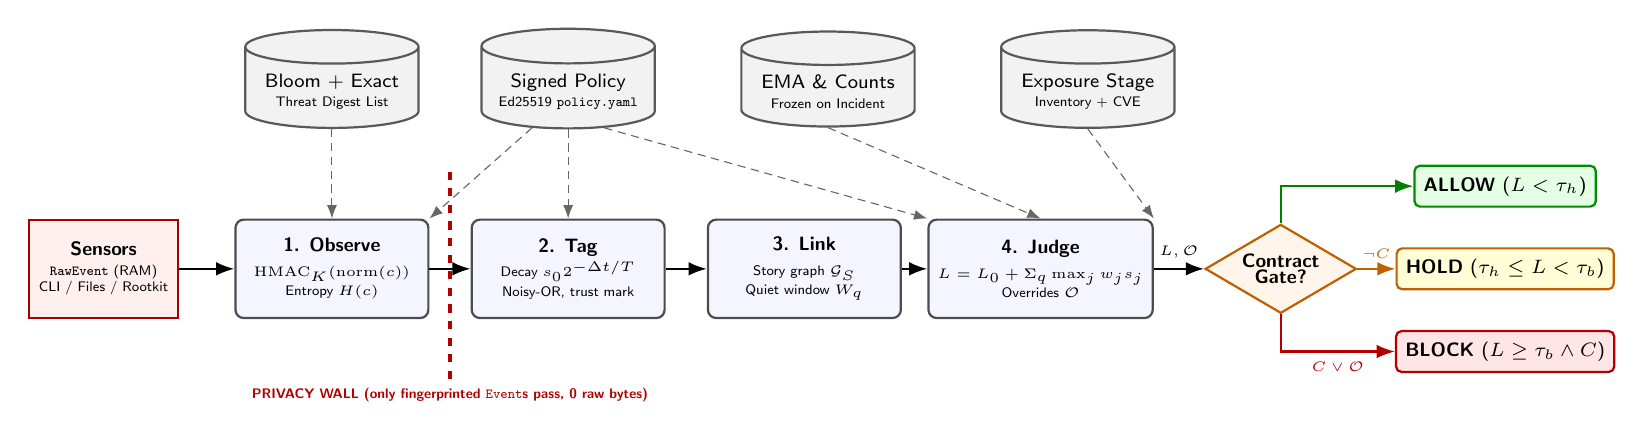
\begin{tikzpicture}[
    font=\scriptsize\sffamily,
    >=Latex,
    stage/.style={rectangle, rounded corners=3pt, draw=black!70, fill=blue!4, thick, minimum width=2.45cm, minimum height=1.25cm, align=center},
    store/.style={cylinder, shape border rotate=90, aspect=0.22, draw=black!65, fill=gray!10, thick, minimum width=2.2cm, minimum height=0.82cm, align=center},
    gate/.style={diamond, aspect=1.7, draw=orange!75!black, fill=orange!8, thick, inner sep=1.5pt, align=center},
    outallow/.style={rectangle, rounded corners=2pt, draw=green!55!black, fill=green!10, thick, minimum width=2.2cm, minimum height=0.52cm, align=center},
    outhold/.style={rectangle, rounded corners=2pt, draw=orange!75!black, fill=yellow!16, thick, minimum width=2.2cm, minimum height=0.52cm, align=center},
    outblock/.style={rectangle, rounded corners=2pt, draw=red!70!black, fill=red!10, thick, minimum width=2.2cm, minimum height=0.52cm, align=center}
  ]
    % Top stores
    \node[store] (bloom) at (0.3, 2.25) {Bloom + Exact\\[-1pt]\tiny Threat Digest List};
    \node[store] (pol) at (3.3, 2.25) {Signed Policy\\[-1pt]\tiny Ed25519 \texttt{policy.yaml}};
    \node[store] (ema) at (6.6, 2.25) {EMA \& Counts\\[-1pt]\tiny Frozen on Incident};
    \node[store] (exp) at (9.9, 2.25) {Exposure Stage\\[-1pt]\tiny Inventory + CVE};

    % Pipeline stages
    \node[rectangle, draw=red!65!black, fill=red!6, thick, minimum width=1.9cm, minimum height=1.25cm, align=center] (raw) at (-2.6, 0) {\textbf{Sensors}\\[-1pt]\tiny \texttt{RawEvent} (RAM)\\[-2pt]\tiny CLI / Files / Rootkit};
    \node[stage] (obs) at (0.3, 0) {\textbf{1. Observe}\\[1pt]\tiny $\mathrm{HMAC}_K(\mathrm{norm}(c))$\\[-1pt]\tiny Entropy $H(c)$};
    \node[stage] (tag) at (3.3, 0) {\textbf{2. Tag}\\[1pt]\tiny Decay $s_0 2^{-\Delta t/T}$\\[-1pt]\tiny Noisy-OR, trust mark};
    \node[stage] (lnk) at (6.3, 0) {\textbf{3. Link}\\[1pt]\tiny Story graph $\mathcal{G}_S$\\[-1pt]\tiny Quiet window $W_q$};
    \node[stage] (jdg) at (9.3, 0) {\textbf{4. Judge}\\[1pt]\tiny $L = L_0 + \Sigma_q \max_j w_j s_j$\\[-1pt]\tiny Overrides $\mathcal{O}$};
    \node[gate] (cgate) at (12.35, 0) {\textbf{Contract}\\[-2pt]\textbf{Gate?}};

    % Decisions
    \node[outallow] (allow) at (15.2, 1.05) {\textbf{ALLOW} ($L < \tau_h$)};
    \node[outhold]  (hold)  at (15.2, 0.0)  {\textbf{HOLD} ($\tau_h \le L < \tau_b$)};
    \node[outblock] (block) at (15.2, -1.05) {\textbf{BLOCK} ($L \ge \tau_b \land C$)};

    % Privacy boundary
    \draw[dashed, very thick, red!70!black] (1.8, -1.4) -- (1.8, 1.25);
    \node[font=\tiny\bfseries\sffamily, text=red!70!black, fill=white, inner sep=1pt] at (1.8, -1.6) {PRIVACY WALL (only fingerprinted \texttt{Event}s pass, 0 raw bytes)};

    % Flow
    \draw[->, thick] (raw) -- (obs);
    \draw[->, thick] (obs) -- (tag);
    \draw[->, thick] (tag) -- (lnk);
    \draw[->, thick] (lnk) -- (jdg);
    \draw[->, thick] (jdg) -- node[above, font=\tiny]{$L, \mathcal{O}$} (cgate);
    \draw[->, thick, green!50!black] (cgate.north) |- (allow.west);
    \draw[->, thick, orange!75!black] (cgate.east) -- node[above, font=\tiny]{$\neg C$} (hold.west);
    \draw[->, thick, red!70!black] (cgate.south) |- node[below, pos=0.75, font=\tiny]{$C \lor \mathcal{O}$} (block.west);

    % Governance
    \draw[->, densely dashed, black!60] (bloom) -- (obs);
    \draw[->, densely dashed, black!60] (pol.south) -- (tag.north);
    \draw[->, densely dashed, black!60] (pol.south west) -- (obs.north east);
    \draw[->, densely dashed, black!60] (pol.south east) -- (jdg.north west);
    \draw[->, densely dashed, black!60] (ema.south) -- (jdg.north);
    \draw[->, densely dashed, black!60] (exp.south) -- (jdg.north east);
  \end{tikzpicture}}
  \caption{Formal TikZ vector schematic of Refmon's mathematical dataflow and shapes: rectangles denote deterministic functional stages, cylinders denote signed/stateful stores, the red dashed boundary marks the irreversible \texttt{Observe} cryptographic wall, and the diamond gate enforces the Contract Gate invariant ($L \ge \tau_{\text{block}} \land \neg C \land \mathcal{O}=\varnothing \implies \text{HOLD}$).}
  \label{fig:tikz_dataflow}
\end{figure*}

\subsection{System Architecture and Core Principles}
\label{sec:arch}

Figures~\ref{fig:pipeline_img} and~\ref{fig:tikz_dataflow} outline Refmon's six-stage pipeline. Sensors monitor system activity in real time and emit structured \texttt{RawEvent} records in memory whenever a notable event occurs, such as executing a program (\texttt{exec}), writing a file (\texttt{file\_write}), or establishing a network connection (\texttt{net\_connect}). Across all supported platforms, Refmon standardizes activity into 13 canonical event types:
\[
\begin{aligned}
\mathcal{T} = \{&\texttt{content\_in}, \texttt{request\_in}, \texttt{request\_end},\\
&\texttt{exec}, \texttt{net\_connect}, \texttt{file\_write}, \texttt{persist},\\
&\texttt{asset\_access}, \texttt{priv\_change}, \texttt{security\_tamper},\\
&\texttt{user\_input}, \texttt{admin\_input}, \texttt{response\_out}\}.
\end{aligned}
\]
Each acting process $a = (\text{id}, \text{parent}, r, \text{interactive}, u)$ carries an assigned workload role $r \in \mathcal{R}$. A role is simply a job description: an interactive terminal has permissions to compile code and run scripts, while a web server worker does not. Refmon provides 16 built-in roles (such as \texttt{interactive\_shell}, \texttt{web\_worker}, \texttt{node\_app\_server}, \texttt{package\_installer}, \texttt{office}, \texttt{launcher}, \texttt{agent}, \texttt{browser}, and \texttt{mail}) and allows administrators to define custom roles (such as \texttt{backup\_job} and \texttt{patch\_tool}).

Two foundational invariants govern the entire pipeline:
\begin{invariant}[Zero Raw Persistence]
\label{inv:raw}
No raw payload $c = o_{\text{raw}}.\text{content}$ or cleartext string (\texttt{domain}, \texttt{host}, \texttt{ip}, \texttt{url\_path}, \texttt{program}, \texttt{signer}) ever crosses the boundary of the \texttt{Observe} stage into persistent storage. All downstream events contain only cryptographic digests and scalar numbers, validated against a strict 21-key allowlist $\mathcal{K}_{\text{allow}}$.
\end{invariant}
\begin{invariant}[Missing Information Neutrality]
\label{inv:missing}
If a sensor lacks the capability to check an attribute (for example, if code-signature verification returns \texttt{signed = "unknown"} or a learned role baseline has not yet gathered enough samples), Refmon treats the signal as neutral ($s_j = 0$) rather than assuming malice. Any such visibility gap is reported out-of-band via the system \texttt{Heartbeat} monitor.
\end{invariant}

\subsection{Stage 1 (\texttt{Observe}): Cryptographic Privacy and Obfuscation Detection}
\label{sec:observe}

When a command or network payload $c \in \Sigma^*$ enters the system, \texttt{Observe} first normalizes whitespace $\tilde{c} = \text{norm}(c)$ and computes an irreversible fingerprint using a 256-bit secret key $K_{\text{dev}}$ stored only on that machine:
\begin{equation}
  f(c) = \texttt{"hmac:"} \,\|\, \operatorname{Hex}\!\Big(\operatorname{HMAC-SHA256}\big(K_{\text{dev}},\, \tilde{c}\big)\Big).
  \label{eq:hmac}
\end{equation}

The cleartext command is then immediately dropped from memory. Before discarding it, if the event involves command execution or user input ($\tau \in \{\texttt{exec},\allowbreak \texttt{content\_in},\allowbreak \texttt{user\_input},\allowbreak \texttt{admin\_input}\}$), \texttt{Observe} calculates three simple statistical shape metrics from the character counts $\{n_x\}$ ($N_c = |c|$, $p_x = n_x / N_c$):
\begin{align}
  H(c) &= -\sum_{x \in \Sigma,\, p_x > 0} p_x \log_2 p_x \quad\text{(bits/char)}, \label{eq:entropy}\\
  \rho_{\text{enc}}(c) &= \frac{1}{N_c}\sum_{i=1}^{N_c} \mathbf{1}\!\left[c_i \in \Sigma_{\text{b64/hex}}\right], \label{eq:encratio}\\
  r_{\text{ws}}(c) &= \max\big\{\ell \in \mathbb{N} : \exists\, i,\; c_{i..i+\ell-1} \in \{\text{' '}, \text{'\textbackslash t'}\}^\ell\big\}. \label{eq:wsrun}
\end{align}
These numbers capture common evasion tricks: high entropy $H(c) > 5.2$~bits reveals encrypted shellcode, a high encoding ratio $\rho_{\text{enc}}$ catches base64-encoded scripts, and long whitespace runs $r_{\text{ws}}(c)$ catch ClickFix tricks (where attackers insert hundreds of spaces so the malicious command is hidden beyond the terminal window's edge). This detection happens entirely in RAM without saving any user commands to disk.

\paragraph{Two-Stage Threat List Matching.} Known malicious threat indicators $\mathcal{D}_{\text{bad}}$ are stored as keyed hashes $d_i = \operatorname{HMAC-SHA256}(K_{\text{list}}, \tilde{v}_i)$ inside an in-memory Bloom filter $\mathcal{B}$ with $m$ bits and $k_h$ hash functions:
\begin{equation}
  m = \left\lceil -\frac{n \ln p_{\text{fp}}}{(\ln 2)^2} \right\rceil, \qquad
  k_h = \max\!\left(1,\, \operatorname{round}\!\left(\frac{m}{n}\ln 2\right)\right),
  \label{eq:bloom}
\end{equation}
configured for a false-positive rate $p_{\text{fp}} \le 10^{-3}$. Any match in the Bloom filter is treated as a fast hint and immediately verified against the exact hash set $\mathcal{D}_{\text{exact}}$, ensuring that the operational threat-list false-positive rate is \emph{strictly zero} (proven in Appendix~\ref{app:privacy}).

\subsection{Stage 2 (\texttt{Tag}): Provenance Tracking, Decay, and Fusion}
\label{sec:tag}

Whenever data arrives from an untrusted source (such as a website download, email attachment, or external network request), Refmon attaches a digital \emph{provenance label} $\ell = (\text{id}, t_0, s_0=1, \text{persistent}, \mathcal{E}_{\text{contract}})$. This label acts as a receipt marking where the data originated.

\paragraph{Half-Life Provenance Decay.} Suspicion naturally fades over time: if a file was downloaded an hour ago and nothing suspicious happened, it should not taint normal user commands forever. Refmon models this using an exponential half-life ($T_{1/2} = 30$~minutes, $\Delta t = t - t_0$):
\begin{equation}
  s_\ell(t) =
  \begin{cases}
    s_0, & \text{if } \ell.\text{pers.} \lor \mathcal{E}_{\text{contract}}(\ell) \neq \varnothing,\\[3pt]
    s_0 \, 2^{-\Delta t / T_{1/2}}, & \text{otherwise.}
  \end{cases}
  \label{eq:decay}
\end{equation}
Crucially, if the process commits a role contract violation ($\mathcal{E}_{\text{contract}}(\ell) \neq \varnothing$), decay immediately freezes. This prevents an attacker from sleeping past $T_{1/2}$ after compromising a process and resuming malicious activity without suspicion.

\paragraph{Edge Attenuation and Noisy-OR Combination.} When a labeled process spawns a child process or writes an intermediate file, the label propagates along the causal edge with attenuation $a_e \in (0, 1]$ ($s_{\text{child}} = a_e \cdot s_{\text{parent}}$). When an action receives untrusted input from several independent sources $\{\ell_1, \dots, \ell_m\}$, Refmon fuses their strengths using Pearl's Noisy-OR model:
\begin{equation}
  s_{\text{comb}}(t) = 1 - \prod_{i=1}^{m} \big(1 - s_{\ell_i}(t)\big).
  \label{eq:noisyor}
\end{equation}
This formula ensures that multiple untrusted inputs increase the overall suspicion, while remaining smoothly bounded between 0 and 1 without artificial saturation. When a labeled process writes an executable to a web directory or sets up a startup script (\texttt{persist}), the file is marked $\text{persistent} = \texttt{true}$, preserving the attack evidence even if the file is executed days later.

\paragraph{Order-Independent Label Hand-Over.} When external content is ingested, the receiving process inherits \emph{every} active label associated with that content, rather than only the strongest one. Because labels combine through Eq.~\eqref{eq:noisyor}, this guarantees that the order of events and slight differences in decay rates never cause Refmon to miss active evidence.

\paragraph{Trusted Lineage and Trust Marks.} Trusted root sources (such as a university's verified software portal) produce no untrusted label. However, in large installations, an installation script may take several minutes to finish. To prevent later steps from being treated as suspicious, a process $p$ that ingests trusted content carries a \emph{trust mark}:
\begin{equation}
  \begin{aligned}
  \operatorname{trust}_p(t) = {}&\mathbf{1}\!\Big[\,2^{-(t - t_p)/T_{1/2}} \ge s_{\text{floor}}\Big]\\
  &\cdot \mathbf{1}\!\Big[\nexists\, \ell \in \operatorname{ever}(p) : s_\ell(t) \ge s_{\text{floor}}\Big],
  \end{aligned}
  \label{eq:trust}
\end{equation}
where $s_{\text{floor}} = 0.02$. The trust mark lasts as long as a normal label would ($\approx 2.8$~hours), passes from parent to child process during the installation, and is instantly cancelled if the lineage ever touches untrusted external content.

\subsection{Stage 3 (\texttt{Link}): Causal Story Grouping}
\label{sec:link}

To distinguish between simultaneous activities, \texttt{Link} groups related events into \emph{causal stories} $\{S_1, S_2, \dots\}$. When a parent process spawns a child, or when a process reads a recently written file within a 10-minute quiet window ($W_q$), the actions are linked into the same story. However, shared programs such as web browsers and email clients are not used as merge keys: opening two separate tabs in a browser maintains two distinct stories, preventing unrelated user downloads from confusing the system.

\subsection{Stage 4 (\texttt{Judge}): Three-Question Bayesian Calculus and Decisions}
\label{sec:judge}

% 1-column TikZ Bayesian Decision Space & Contract Gate Shape Diagram
\begin{figure}[!t]
  \centering
  \resizebox{\columnwidth}{!}{%
    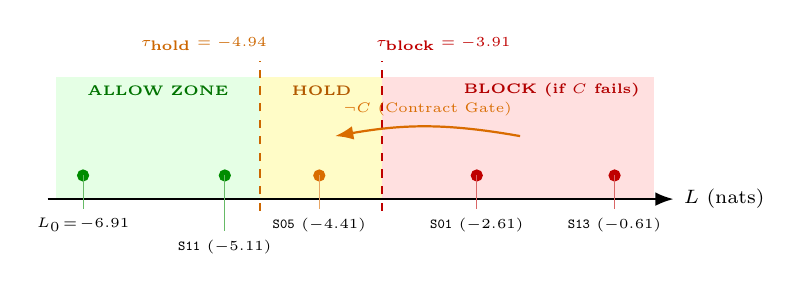
\begin{tikzpicture}[font=\scriptsize\sffamily, >=Latex]
    % Background zones
    \fill[green!10] (0, 0) rectangle (2.6, 1.55);
    \fill[yellow!22] (2.6, 0) rectangle (4.15, 1.55);
    \fill[red!12] (4.15, 0) rectangle (7.6, 1.55);

    % Axis and thresholds
    \draw[->, thick] (-0.1, 0) -- (7.85, 0) node[right, font=\scriptsize]{$L$ (nats)};
    \draw[dashed, thick, orange!80!black] (2.6, -0.15) -- (2.6, 1.75) node[above left=0pt and -6pt, font=\tiny\bfseries]{$\tau_{\text{hold}}=-4.94$};
    \draw[dashed, thick, red!75!black] (4.15, -0.15) -- (4.15, 1.75) node[above right=0pt and -6pt, font=\tiny\bfseries]{$\tau_{\text{block}}=-3.91$};

    % Zone labels
    \node[font=\tiny\bfseries, text=green!45!black] at (1.3, 1.38) {ALLOW ZONE};
    \node[font=\tiny\bfseries, text=orange!70!black] at (3.38, 1.38) {HOLD};
    \node[font=\tiny\bfseries, text=red!70!black] at (6.3, 1.38) {BLOCK (if $C$ fails)};

    % Scenario points (labels below the axis, two rows)
    \foreach \px/\py/\pc/\pl in {0.35/-0.22/green!55!black/{$L_0\!=\!-6.91$}, 2.15/-0.5/green!55!black/{\texttt{S11} ($-5.11$)}, 3.35/-0.22/orange!85!black/{\texttt{S05} ($-4.41$)}, 5.35/-0.22/red!75!black/{\texttt{S01} ($-2.61$)}, 7.10/-0.22/red!75!black/{\texttt{S13} ($-0.61$)}} {
      \filldraw[\pc] (\px, 0.3) circle (2pt);
      \draw[\pc!60, thin] (\px, 0.3) -- (\px, \py+0.1);
      \node[font=\tiny, anchor=north] at (\px, \py+0.1) {\pl};
    }

    % Contract gate
    \draw[->, thick, bend right=10, orange!85!black] (5.9, 0.8) to node[above, font=\tiny]{$\neg C$ (Contract Gate)} (3.55, 0.8);
  \end{tikzpicture}}
  \caption{Bayesian log-odds decision geometry showing prior $L_0 = -6.91$~nats, cost thresholds $\tau_{\text{hold}} = -4.94$ and $\tau_{\text{block}} = -3.91$, benchmark trajectories (\texttt{S11} pasted benign echo, \texttt{S05} hand-typed fetch, \texttt{S01} ClickFix, \texttt{S13} web RCE), and the Contract Gate projection.}
  \label{fig:tikz_thresholds}
\end{figure}

For each story $S$, let $s_{\text{ori}}(S) = \max_{\ell \in \mathcal{L}(S)} s_\ell(t_{\text{last}})$ denote the strongest active provenance label. The \texttt{Judge} evaluates every sequence of actions by answering three concrete, intuitive questions $\mathcal{Q} = \{\text{origin}, \text{contract}, \text{effect}\}$:
\begin{itemize}[leftmargin=1.3em,itemsep=1.5pt,topsep=2pt]
  \item \textbf{Question 1: Origin ($Q_{\text{origin}}$).} Did this sequence of actions originate from an untrusted external source? It fails if the active label strength $s_{\text{ori}}(S) \ge \theta_{\text{ori}}$ ($0.5$), yielding signal \texttt{origin\_external}.
  \item \textbf{Question 2: Contract ($Q_{\text{contract}}$).} Did the acting process violate its declared job description? It fails if the action violates a role contract (such as a web server spawning a shell), breaches a universal policy rule, or exhibits high statistical surprisal in a mature baseline.
  \item \textbf{Question 3: Effect ($Q_{\text{effect}}$).} Did the action attempt a hazardous operation? It fails if the process attempts dangerous operations like reading credentials, encrypting files, or connecting to unauthorized external endpoints.
\end{itemize}
Connections to trusted destinations (such as package repositories) do not raise network effect signals for normal processes. Since \texttt{v1.5} (A60), this exception applies only if the process lineage has never touched an untrusted external label, preventing attackers from abusing trusted hosts to bypass detection.

\paragraph{Max-Sum Bayesian Log-Odds Calculus.} Each detected signal $j$ carries a log-likelihood ratio weight:
\begin{equation}
  w_j = \ln \frac{\mathbb{P}(j \mid \text{attack})}{\mathbb{P}(j \mid \text{benign})} \quad (\text{in nats}),
  \label{eq:llr_weight}
\end{equation}
reflecting how much more frequently that signal appears in genuine attacks compared to normal operations (Table~\ref{tab:weights}). When re-estimating weights from empirical corpora, Laplace smoothing ensures stability:
\begin{equation}
  \hat{w}_j = \ln \frac{(a_j + 1)/(|\mathcal{A}| + 2)}{(b_j + 1)/(|\mathcal{B}| + 2)}.
  \label{eq:reestimate}
\end{equation}

If an event triggers three overlapping network heuristics, simply adding their weights would unfairly triple the suspicion score. To avoid this, Refmon takes the \textbf{maximum} signal within each question, and \textbf{sums} across the three independent questions. Starting from a prior attack probability $\pi = 10^{-3}$ ($L_0 = \ln\frac{\pi}{1-\pi} \approx -6.91$~nats), the posterior log-odds for story $S$ is:
\begin{equation}
  L(S) = \ln\frac{\pi}{1 - \pi} + \sum_{q \in \{\text{origin},\,\text{contract},\,\text{effect}\}} \;\max_{j \in \mathcal{S}_q(S)} \big(w_j \cdot s_j\big),
  \label{eq:logodds}
\end{equation}
with empty question maxima defaulting to $0$. The posterior attack probability is $\mathbb{P}(\text{attack} \mid S) = \sigma(L(S)) = (1 + e^{-L(S)})^{-1}$. In \texttt{v1.3} (Decision A55), only $Q_{\text{origin}}$ scales with decaying label strength $s_{\text{ori}}(S)$, while Contract and Effect signals use fixed unit strength ($s_j = 1$). This guarantees that overall suspicion $L(S)$ increases monotonically with label strength (Theorem~\ref{thm:monotone}, Appendix~\ref{app:monotone}).

\paragraph{Cost-Optimal Thresholds and the Contract Gate.} Let $C_{\text{miss}}$ ($1000$), $C_{\text{fb}}$ ($20$), and $C_{\text{hold}}$ ($5$) represent the operational costs of missing an attack, making a false block, or holding a job for human review, and let $h = 0.7$ be the probability that a hold stops an attack. Applying Bayes minimal-risk decision theory (Appendix~\ref{app:bayes}) yields two exact log-odds thresholds:
\begin{equation}
  \tau_{\text{block}} = \ln\frac{C_{\text{fb}}}{C_{\text{miss}}} \approx -3.91,\quad
  \tau_{\text{hold}} = \ln\frac{C_{\text{hold}}}{h C_{\text{miss}}} \approx -4.94.
  \label{eq:thresholds}
\end{equation}

Before applying these thresholds, four high-priority overrides $\mathcal{O}$ run in strict order: tampering with Refmon (\texttt{OVR-SELF-TAMPER} $\mapsto \texttt{BLOCK}$), tripping canary files (\texttt{OVR-CANARY} $\mapsto \texttt{BLOCK}$), accessing protected secrets while carrying an untrusted label (\texttt{OVR-PROTECTED-ASSET} $\mapsto \texttt{BLOCK}$), or running signed code from a trusted root (\texttt{OVR-TRUSTED-ROOT} $\mapsto \texttt{ALLOW}$).

When no override applies, Refmon enforces the \textbf{Contract Gate} (Figure~\ref{fig:tikz_thresholds}):
\begin{equation}
  D(S) =
  \begin{cases}
    \texttt{BLOCK}, & \text{if } L(S) \ge \tau_{\text{block}} \;\land\; Q_{\text{contract}}(S),\\
    \texttt{HOLD},  & \text{if } \big(L(S) \ge \tau_{\text{block}} \;\land\; \neg Q_{\text{contract}}(S)\big)\\
                    & \quad\;\lor\; \big(\tau_{\text{hold}} \le L(S) < \tau_{\text{block}}\big),\\
    \texttt{ALLOW}, & \text{if } L(S) < \tau_{\text{hold}}.
  \end{cases}
  \label{eq:decide}
\end{equation}
The Contract Gate establishes a critical safety invariant: \textbf{Refmon never blocks an action outright unless a signed role contract was broken.} Even if an action looks unusual ($L(S) \ge \tau_{\text{block}}$), if it stayed within its allowed role permissions, it is placed on \texttt{HOLD} for human review rather than being abruptly terminated.

\subsection{Contract Surprisal and Baseline Maturity}
\label{sec:rarity}

When learning baseline behaviors for a role $r$, let $n_{r,e}$ be the observed count of behavior $e$, $N_r = \sum n_{r,e}$ the total observations over $K_r$ distinct behaviors, and $n_{r,1}$ the number of behaviors seen exactly once. Using Laplace smoothing ($\alpha = 1$) to reserve probability mass for previously unseen behaviors, the smoothed probability and Shannon surprisal are:
\begin{equation}
  \hat{p}(e \mid r) = \frac{n_{r,e} + \alpha}{N_r + \alpha(K_r + 1)}, \quad
  I(e \mid r) = -\log_2 \hat{p}(e \mid r).
  \label{eq:surprisal}
\end{equation}
A newly deployed system might encounter normal developer commands it has not seen before. To uphold Invariant~\ref{inv:missing} and prevent false alarms during initial startup, surprisal signals ($I(e \mid r) \ge 12$~bits) remain inactive until the Good-Turing estimate of unseen probability mass drops below $1\%$ ($\tau_{\text{mat}} = 0.01$):
\begin{equation}
  \hat{p}_{\text{unseen}}(r) = \frac{n_{r,1}}{N_r} < \tau_{\text{mat}}.
  \label{eq:goodturing}
\end{equation}

\subsection{Dual-Window Burst and Drift Detection}
\label{sec:rates}

To catch attacks like ransomware or slow data exfiltration, Refmon tracks activity rates over both a short window ($60$~seconds) and a long window ($1$~hour):
\begin{enumerate}[leftmargin=1.4em,itemsep=1.5pt,topsep=2pt]
  \item \textbf{Poisson Upper-Tail Burst Test (\texttt{mass\_change}, \texttt{lateral}):} Given baseline rate $\hat{\lambda}$ and $k$ operations in the window, an alert fires if the burst probability is negligible:
  \begin{equation}
    \mathbb{P}(X \ge k \mid \operatorname{Pois}(\hat{\lambda})) = \sum_{i=k}^{\infty} \frac{e^{-\hat{\lambda}}\hat{\lambda}^i}{i!} < 10^{-6}.
    \label{eq:poisson}
  \end{equation}
  \item \textbf{CUSUM Drift Test (\texttt{exfil} volume):} For outbound data volume $x_t$ with mean $\mu_r$ and standard deviation $\sigma_r$, the standardized score $z_t = (x_t - \mu_r)/\sigma_r$ is tracked with slack $k_c = 0.5$ and threshold $h_c = 5.0$:
  \begin{equation}
    S_t = \max\big(0,\, S_{t-1} + z_t - k_c\big), \qquad \text{alert iff } S_t > h_c.
    \label{eq:cusum}
  \end{equation}
\end{enumerate}
All moving-average baselines freeze automatically when an incident is open on a process tree, preventing an attacker from poisoning normal baselines. The incident closes and baselines unfreeze once the process tree has been silent for a full hour ($1$~h), ensuring long-term stability.

\subsection{Six-Engine Cross-View Rootkit Detection}
\label{sec:rootkit}

Refmon detects stealth implants in user space without requiring root privileges by running $m \ge 2$ passes across six read-only engines: (E1)~dynamic linker preloads (\texttt{/etc/ld.so.preload}, \texttt{LD\_PRELOAD}), (E2)~fileless execution and memory injection (\texttt{memfd:}, deleted binaries, anonymous \texttt{rwxp} pages), (E3)~hidden kernel module cross-view (\texttt{/sys/module} $\setminus$ \texttt{/proc/modules}), (E4)~hidden PID cross-view (\texttt{/proc} directory scans versus direct process checks), (E5)~socket cross-view and sniffer detection (\texttt{/proc/net/sockstat} versus \texttt{/proc/net/tcp}), and (E6)~optional verification using external tools if installed.

To eliminate false alarms caused by short-lived processes exiting mid-scan, Refmon requires discrepancies to persist across all $m$ passes:
\begin{equation}
  \Delta_{\text{pers}} = \bigcap_{r=1}^{m} \Big(\mathcal{V}_{\text{low}}^{(r)} \setminus \mathcal{V}_{\text{high}}^{(r)}\Big).
  \label{eq:crossview_intersect}
\end{equation}
Confirmed persistent findings map directly to log-odds evidence:
\begin{equation}
  w_{\text{rk}}(d, m) = \min\!\Big(w_{\max},\; \ln\frac{p_{\text{tp}}}{p_{\text{race}}} + (m - 1)\ln\frac{1}{q_{\text{persist}}}\Big),
  \label{eq:rk_nats}
\end{equation}
suppressing transient operating system churn while providing decisive detection of genuine stealth rootkits.

\subsection{Stages 5 \& 6 (\texttt{Gate}, \texttt{Contain}, \texttt{Exposure}, \texttt{Report})}
\label{sec:gate}

% 1-column TikZ Hold & Containment State Machine Shape Diagram
\begin{figure}[!t]
  \centering
  \resizebox{\columnwidth}{!}{%
    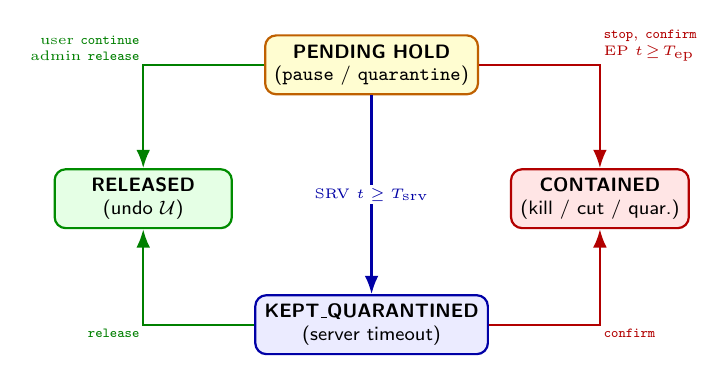
\begin{tikzpicture}[
    font=\scriptsize\sffamily,
    >=Latex,
    st/.style={rectangle, rounded corners=4pt, draw=black!70, fill=gray!8, thick, minimum width=2.25cm, minimum height=0.62cm, align=center},
    stbad/.style={rectangle, rounded corners=4pt, draw=red!70!black, fill=red!10, thick, minimum width=2.25cm, minimum height=0.62cm, align=center},
    stgood/.style={rectangle, rounded corners=4pt, draw=green!55!black, fill=green!10, thick, minimum width=2.25cm, minimum height=0.62cm, align=center},
    lbl/.style={font=\tiny, fill=white, inner sep=1pt}
  ]
    \node[st, fill=yellow!18, draw=orange!75!black] (pend) at (0, 0) {\textbf{PENDING HOLD}\\(\texttt{pause} / \texttt{quarantine})};
    \node[stgood] (rel) at (-2.9, -1.7) {\textbf{RELEASED}\\(undo $\mathcal{U}$)};
    \node[stbad] (cont) at (2.9, -1.7) {\textbf{CONTAINED}\\(kill / cut / quar.)};
    \node[st, fill=blue!8, draw=blue!65!black] (kept) at (0, -3.3) {\textbf{KEPT\_QUARANTINED}\\(server timeout)};

    \draw[->, thick, green!50!black] (pend.west) -| node[lbl, pos=0.5, anchor=south east, align=right]{user \texttt{continue}\\admin \texttt{release}} (rel.north);
    \draw[->, thick, red!70!black] (pend.east) -| node[lbl, pos=0.5, anchor=south west, align=left]{\texttt{stop}, \texttt{confirm}\\EP $t\!\ge\!T_{\text{ep}}$} (cont.north);
    \draw[->, thick, blue!65!black] (pend.south) -- node[lbl]{SRV $t \ge T_{\text{srv}}$} (kept.north);
    \draw[->, thick, green!50!black] (kept.west) -| node[lbl, pos=0.5, anchor=north east]{\texttt{release}} (rel.south);
    \draw[->, thick, red!70!black] (kept.east) -| node[lbl, pos=0.5, anchor=north west]{\texttt{confirm}} (cont.south);
  \end{tikzpicture}}
  \caption{Dual endpoint vs.\ server hold state machine in \texttt{Gate}. Endpoint timeouts fail closed into containment, whereas unattended server holds preserve service stability in \texttt{KEPT\_QUARANTINED} until an administrator decides.}
  \label{fig:tikz_hold_fsm}
\end{figure}

Figure~\ref{fig:tikz_hold_fsm} illustrates how \texttt{Gate} enforces decisions across three operating modes: \texttt{observe} (logs decisions without acting), \texttt{warn} (notifies users without blocking), and \texttt{block} (actively enforces policy).

When an attack is detected, Refmon takes targeted containment actions:
\begin{itemize}[leftmargin=1.3em,itemsep=1.5pt,topsep=2pt]
  \item \textbf{Process Termination (\texttt{kill\_process\_tree}):} Safely terminates the offending process and any child processes it spawned.
  \item \textbf{Network Isolation (\texttt{cut\_network}):} Closes suspicious active sockets.
  \item \textbf{File Quarantine (\texttt{quarantine\_file}):} Moves suspicious dropped files (such as web shells) into a protected quarantine directory with read-only permissions (\texttt{mode 0400}) rather than deleting them, preserving evidence for human analysis.
\end{itemize}
All containment actions generate reversible undo tokens $\mathcal{U}$, allowing an administrator to restore an action with a single command if needed. Containment targets only labeled processes and files; interactive developer shells and shared applications (like browsers) are never terminated directly.

\paragraph{Dual Endpoint vs.\ Server Timeout Handling.} As shown in Figure~\ref{fig:tikz_hold_fsm}, unattended servers handle held jobs differently from interactive workstations. On an interactive workstation, an unanswered prompt eventually times out and halts the suspicious process. On an unattended production server, an unanswered hold moves the affected file into a safe holding state (\texttt{KEPT\_QUARANTINED}) while keeping the main service running, ensuring server stability until an administrator investigates.

\paragraph{Privacy-Preserving Fleet Reporting.} To report fleet-wide security trends without exposing individual user habits, Refmon adds calibrated Laplace noise $\tilde{c} = c + \operatorname{Lap}(1/\varepsilon)$ ($\varepsilon$-differential privacy) to aggregated counts, suppresses reporting groups with fewer than $k = 5$ devices ($k$-anonymity), and enforces a strict four-eyes rule: unmasking any device pseudonym requires cryptographic signatures from two distinct human administrators recorded on a tamper-evident audit log.

% ============================================================================
% 4. EXPERIMENTS, ALGORITHMS, AND IMPLEMENTATION TESTS
% ============================================================================
\section{Experiments, Algorithms, and Implementation Tests}
\label{sec:eval}

\subsection{Reference Implementation and Signed Policy Governance}
\label{sec:impl}

Refmon is implemented in approximately 12,400 lines of strict, type-checked Python~3.12 (plus 10,200 lines of tests) (\texttt{pydantic} v2 frozen schemas, \texttt{cryptography} Ed25519 signatures, zero runtime machine-learning dependencies). Every threshold, weight, role contract, canary, and rate parameter resides in a canonical JSON-serialized, Ed25519-signed \texttt{policy.yaml}; startup and live reload reject any unsigned or tampered policy (\texttt{PolicyRejected}) and retain the last verified state. A periodic \texttt{SelfTest} scheduler clones the live pipeline via \texttt{pipeline.probe()} (preserving live disabled rules and weights while isolating outputs) to inject synthetic health stories and raise immediate alerts if any enabled protection fails to reach its expected decision.

\subsection{Core Pipeline and Scanner Algorithms}
\label{sec:algorithms}

Algorithms~\ref{alg:pipeline}, \ref{alg:judge}, and~\ref{alg:rootkit} specify the exact deterministic execution of the Refmon event loop, the monotone Bayesian \texttt{Judge}, and the multi-pass cross-view rootkit sensor. Listing~\ref{lst:barrier} (Appendix~\ref{app:supplementary}) shows the unprivileged command-barrier loop from \texttt{src/refmon/live.py}.

\begin{algbox}{End-to-End Refmon Event Processing (\texttt{Pipeline.process})}{alg:pipeline}
  \item \textbf{Input:} Sensor event $e_{\text{raw}} \in \texttt{RawEvent} \cup \texttt{Event}$, verified policy $\Pi$, device HMAC key $K_{\text{dev}}$.
  \item \textbf{Output:} Emitted verdicts and containment actions $\mathcal{V} \subseteq \texttt{Verdict} \cup \texttt{Action}$.
  \item $e \leftarrow \textsc{Observe}(e_{\text{raw}}, \Pi, K_{\text{dev}})$ \hfill $\triangleright$ Compute $\text{HMAC}_{K_{\text{dev}}}$, $H(c)$, Bloom+Exact check; drop raw content
  \item $p_{\text{known}} \leftarrow (e.\text{actor.parent} \in \text{Tagger.procs})$
  \item $\text{tg} \leftarrow \textsc{Tag}(e, \Pi)$ \hfill $\triangleright$ Apply propagation rules 1--7, decay $2^{-\Delta t / T_{1/2}}$, Noisy-OR
  \item $(\mathcal{S}, \mathcal{F}) \leftarrow \textsc{ExtractSignals}(e, \text{tg}, \Pi, \text{Rates}, \text{Baseline})$
  \item $\text{rec} \leftarrow \textsc{Link}(\text{tg}, p_{\text{known}}, \mathcal{S}, \mathcal{F}, \Pi)$ \hfill $\triangleright$ Assign/merge story within quiet window $W_q$
  \item $J \leftarrow \textsc{Judge}(\text{rec}, \text{Tagger}, \Pi)$ \hfill $\triangleright$ Algorithm~\ref{alg:judge}
  \item $\text{Rates.mark\_incident}(\text{root}(e.\text{actor}),\, J.\text{decision} \neq \texttt{ALLOW},\, e.\text{ts})$ \hfill $\triangleright$ Freeze baselines; end incidents silent for 1~h
  \item \textbf{if} $\{s \in J.\text{signals} : s.\text{question}=\text{contract} \land \neg s.\text{carried}\} \neq \varnothing$ \textbf{then}
  \item \hspace{1.0em} Freeze decay and attach contract evidence to active labels $\ell \in \text{rec.label\_ids}$
  \item $\mathcal{V} \leftarrow \textsc{EmitVerdictIfChanged}(\text{rec}, J)$
  \item \textbf{if} $\text{Gate} \neq \texttt{None}$ \textbf{then} $\mathcal{V} \leftarrow \text{Gate.tick}(e.\text{ts}) \,\|\, \mathcal{V} \,\|\, \text{Gate.handle}(\text{rec}, J, e.\text{ts})$
  \item \textbf{return} $\mathcal{V}$
\end{algbox}

\begin{algbox}{Monotone Question-Grouped Bayesian Judge (\texttt{v2.0})}{alg:judge}
  \item \textbf{Input:} Story record $\text{rec}$, provenance tagger $\mathcal{T}$, signed policy $\Pi$.
  \item \textbf{Output:} Story judgement $J = (\text{decision}, L, \text{failed}, \text{override}, \text{gated})$.
  \item $s_{\text{ori}} \leftarrow \max_{\ell \in \text{rec.label\_ids}} \mathcal{T}.\text{strength}(\ell, \text{rec.last\_ts})$; \quad $\text{labeled} \leftarrow (s_{\text{ori}} \ge \Pi.\theta_{\text{ori}}) \land \Pi.\text{enabled}(\texttt{R-ORI})$
  \item Filter $\mathcal{S} \leftarrow \{s \in \text{rec.signals} : (\neg s.\text{allowed} \lor \text{labeled}) \land \Pi.\text{rule\_enabled}(s) \land s \notin \Pi.\text{exceptions}\}$
  \item Append persistent carried contract signals from $\{\ell \in \text{rec.label\_ids} : s_\ell \ge \Pi.\theta_{\text{ori}}\}$
  \item Check priority overrides $\mathcal{O}$: \texttt{self\_tamper} $\succ$ \texttt{canary} $\succ$ \texttt{protected\_asset} $\mapsto \texttt{BLOCK}$; unlabeled \texttt{trusted} (source event or live trust mark) $\mapsto \texttt{ALLOW}$
  \item \textbf{if} $\mathcal{O} \neq \texttt{None}$ \textbf{then return} forced override decision with audit trace
  \item $\mathcal{E} \leftarrow \{(s.\text{question}, s.\text{name}, 1.0) : s \in \mathcal{S}\}$ \hfill $\triangleright$ \texttt{v1.3}: unit strength for Contract \& Effect
  \item \textbf{if} $\text{labeled}$ \textbf{then} $\mathcal{E} \leftarrow \mathcal{E} \cup \{(\text{origin}, \texttt{origin\_external}, s_{\text{ori}})\}$
  \item $L \leftarrow \ln\frac{\Pi.\pi}{1 - \Pi.\pi} + \sum_{q \in \{\text{ori},\text{con},\text{eff}\}} \max_{(q, j, s_j) \in \mathcal{E}} (\Pi.w_j \cdot s_j)$
  \item $\tau_b \leftarrow \ln(\Pi.C_{\text{fb}} / \Pi.C_{\text{miss}})$; \quad $\tau_h \leftarrow \ln(\Pi.C_{\text{hold}} / (\Pi.h \cdot \Pi.C_{\text{miss}}))$; \quad $C_{\text{fail}} \leftarrow \exists s \in \mathcal{S}: s.\text{question}=\text{contract}$
  \item \textbf{if} $L \ge \tau_b \land C_{\text{fail}}$ \textbf{then return} $(\texttt{BLOCK}, L, \text{gated}=\texttt{false})$
  \item \textbf{else if} $L \ge \tau_b \land \neg C_{\text{fail}}$ \textbf{then return} $(\texttt{HOLD}, L, \text{gated}=\texttt{true})$ \hfill $\triangleright$ Contract Gate
  \item \textbf{else if} $L \ge \tau_h$ \textbf{then return} $(\texttt{HOLD}, L, \text{gated}=\texttt{false})$
  \item \textbf{else return} $(\texttt{ALLOW}, L, \text{gated}=\texttt{false})$
\end{algbox}

\begin{algbox}{Multi-Pass 6-Engine Read-Only Rootkit Cross-View Sensor}{alg:rootkit}
  \item \textbf{Input:} Pass count $m \ge 2$, interval $\Delta\tau$, own UID $u$, signed policy $\Pi$.
  \item \textbf{Output:} Structured \texttt{RootkitScanReport} with posterior $L_{\text{rk}}$ and decision $D_{\text{rk}}$.
  \item $\mathcal{F}_{\text{single}} \leftarrow \textsc{ScanPreloadAndMemfdAndMaps}(u) \cup \textsc{ScanTaintAndPromisc}()$
  \item \textbf{for} $r = 1 \dots m$ \textbf{do}
  \item \hspace{1.0em} $\Delta_{\text{mod}}^{(r)} \leftarrow \textsc{SysfsModules}() \setminus \textsc{ProcModules}()$ \hfill $\triangleright$ Engine 4: Hidden LKM check
  \item \hspace{1.0em} $\Delta_{\text{pid}}^{(r)} \leftarrow \textsc{DirectOwnPidProbe}(u) \setminus \textsc{ProcReaddirPids}()$ \hfill $\triangleright$ Engine 6: Hidden PID check
  \item \hspace{1.0em} \textbf{if} $r < m$ \textbf{then} sleep($\Delta\tau$)
  \item $\Delta_{\text{mod}}^* \leftarrow \bigcap_{r=1}^{m} \Delta_{\text{mod}}^{(r)}$; \quad $\Delta_{\text{pid}}^* \leftarrow \bigcap_{r=1}^{m} \Delta_{\text{pid}}^{(r)}$ \hfill $\triangleright$ Suppress transient churn
  \item Map $\mathcal{F} \leftarrow \mathcal{F}_{\text{single}} \cup \textsc{Findings}(\Delta_{\text{mod}}^*, \Delta_{\text{pid}}^*)$ to log-odds $L_{\text{rk}} = L_0 + \sum_{f \in \mathcal{F}} w_{\text{rk}}(f, m)$
  \item Evaluate $D_{\text{rk}} \leftarrow \textsc{Decide}(L_{\text{rk}}, \tau_b, \tau_h, \text{override}=\texttt{SELF\_TAMPER if } \exists f.\text{self\_tamper})$
  \item \textbf{return} $\texttt{RootkitScanReport}(\mathcal{F}, L_{\text{rk}}, D_{\text{rk}})$
\end{algbox}

\subsection{Golden Catalog and Seeded Mutation Robustness}
\label{sec:golden_results}

\paragraph{Strict Pre-Registration Testing Protocol.} To guarantee that our benchmarks were completely unbiased and free of cherry-picking, all signal weights (Table~\ref{tab:weights}) and structural rules were frozen before catalog evaluation and remained unchanged throughout. To test resilience against evasions, we used an automated generator to produce hundreds of realistic variations from pre-registered random seeds. The generator systematically mutated six dimensions: delivery channel, launcher program, obfuscation technique, network target, process tree depth, and timing intervals between actions. Across the initial release tags (\texttt{v1.0} through \texttt{v1.3}), 879 mutated event streams were evaluated using pre-registered seed \texttt{654514256}, ensuring identical, fair test inputs across all versions.

\begin{table*}[!t]
  \centering
  \caption{Robustness Evaluation Across Specification Versions \texttt{v1.0}--\texttt{v1.3} on 46 Golden Scenarios and 879 Seeded Variants (Seed \texttt{654514256}), with Wilson 95\% Confidence Intervals~\cite{wilson1927probable} and Paired Exact McNemar Tests~\cite{mcnemar1947note}.}
  \label{tab:results_matrix}
  \resizebox{\textwidth}{!}{%
  \begin{tabular}{@{}lrrrr@{}}
    \toprule
    \textbf{Evaluation Metric / Benchmark Partition} & \textbf{\texttt{v1.0} (Frozen)} & \textbf{\texttt{v1.1} (A46--A50)} & \textbf{\texttt{v1.2} (A51--A54)} & \textbf{\texttt{v1.3} (Monotone)} \\
    \midrule
    Golden Catalog Scenarios Matching Expected Decision ($N = 46$) & $46/46$ ($100.0\%$) & $46/46$ ($100.0\%$) & $46/46$ ($100.0\%$) & \textbf{$46/46$ ($100.0\%$)} \\
    \midrule
    \textbf{Malicious Variants ($N = 633$)} & & & & \\
    \quad Blocked outright & $425$ ($67.1\%$) & $467$ ($73.8\%$) & $467$ ($73.8\%$) & \textbf{$486$ ($76.8\%$)} \\
    \quad Effective Hold (process paused / file quarantined) & $121$ ($19.1\%$) & $157$ ($24.8\%$) & $157$ ($24.8\%$) & $139$ ($22.0\%$) \\
    \quad Contained = Block + Effective Hold [Wilson 95\% CI] & $86.3\%$ [$83.4, 88.7$] & $98.6\%$ [$97.3, 99.3$] & $98.6\%$ [$97.3, 99.3$] & \textbf{$98.7\%$ [$97.5, 99.4$]} \\
    \quad Caught = Block + Any Hold [Wilson 95\% CI] & $97.2\%$ [$95.6, 98.2$] & $98.6\%$ [$97.3, 99.3$] & $98.6\%$ [$97.3, 99.3$] & \textbf{$98.7\%$ [$97.5, 99.4$]} \\
    \quad Uncontained: Hold that paused nothing & $69$ & $0$ & $0$ & \textbf{$0$} \\
    \quad Uncontained: Allowed malicious variants (Gaps G1--G3) & $18$ & $9$ & $9$ & \textbf{$8$} \\
    \quad Blocks that acted on nothing (unlabeled fallback gap) & $11$ & $9$ & $0$ & \textbf{$0$} \\
    \midrule
    \textbf{Independent Seed-Decided Malicious Subset ($N = 322$)} & & & & \\
    \quad Contained (Block + Effective Hold) & $269/322$ ($83.5\%$) & $313/322$ ($97.2\%$) & $313/322$ ($97.2\%$) & \textbf{$314/322$ ($97.5\%$)} \\
    \midrule
    \textbf{Neutral Benign Variants ($N = 151$, False-Alarm Test)} & & & & \\
    \quad Allowed / Held / False-Blocked & $126$ / $22$ / $3$ & $126$ / $22$ / $3$ & $126$ / $22$ / $3$ & $125$ / $23$ / $3$ \\
    \quad Neutral False-Block Rate [Wilson 95\% CI] & $2.0\%$ [$0.7, 5.7$] & $2.0\%$ [$0.7, 5.7$] & $2.0\%$ [$0.7, 5.7$] & \textbf{$2.0\%$ [$0.7, 5.7$]} \\
    \midrule
    \textbf{Paired McNemar Exact Test vs.\ \texttt{v1.3} (Malicious, $N = 633$)} & & & & \\
    \quad Contained: $(\text{only baseline},\, \text{only \texttt{v1.3}})$, exact $p$-value & $(0, 79),\; p = 3.3\!\times\!10^{-24}$ & $(0, 1),\; p = 1.0$ & $(0, 1),\; p = 1.0$ & --- \\
    \quad Blocked: $(\text{only baseline},\, \text{only \texttt{v1.3}})$, exact $p$-value & $(0, 61),\; p = 8.7\!\times\!10^{-19}$ & $(0, 19),\; p = 3.8\!\times\!10^{-6}$ & $(0, 19),\; p = 3.8\!\times\!10^{-6}$ & --- \\
    \bottomrule
  \end{tabular}}
\end{table*}

Table~\ref{tab:results_matrix} summarizes the progression from \texttt{v1.0} to \texttt{v1.3}. All 46 golden scenarios across all 17 attack families reach their exact expected decisions ($100\%$). Across the 633 malicious variants, fixing hold containment on unlabeled signal-producing processes (\texttt{v1.1}--\texttt{v1.2}) eliminated all 69 ``holds that paused nothing'' and all 11 ``blocks that acted on nothing,'' raising active containment from $86.3\%$ to $98.7\%$ ($p = 3.3 \times 10^{-24}$). Enforcing monotonicity in \texttt{v1.3} converted 19 faded-label holds into decisive blocks ($p = 3.8 \times 10^{-6}$ vs.\ \texttt{v1.2}) while keeping the false-block rate on neutral benign mutations unchanged at $2.0\%$ ($3/151$).

\begin{table*}[!t]
  \centering
  \caption{Pre-Registered Rounds \texttt{v1.4}$\to$\texttt{v2.0}. Each round replays one fresh seed's variants through the version before and after the change. ``Contained'' = block + hold that paused, quarantined or killed something; Wilson 95\% intervals; neutral benign variants carry no mutation the specification forbids.}
  \label{tab:rounds}
  \footnotesize
  \begin{tabularx}{\textwidth}{@{}ll>{\raggedright\arraybackslash}Xlll@{}}
    \toprule
    \textbf{Round} & \textbf{Seed} & \textbf{Structural change (design decision; motivating finding)} & \textbf{Contained, before $\to$ after} & \textbf{Neutral false blocks} & \textbf{Benign changed} \\
    \midrule
    \texttt{v1.4}$\to$\texttt{v1.5} & \texttt{833754500} & lineage-aware destination trust, incidents end, bounded state (A60--A62; F2) & $630 \to 631/637$, $99.1\%$ [$98.0, 99.6$] & $1/158$ ($0.6\%$) & none \\
    \texttt{v1.5}$\to$\texttt{v1.6} & \texttt{545728926} & labeled block with no labeled process acts on its producers (A63; F11) & $623 \to 624/636$, $98.1\%$ [$96.7, 98.9$] & $1/161$ ($0.6\%$) & none \\
    \texttt{v1.6}$\to$\texttt{v1.7} & \texttt{616687759} & every live label handed over (A64; property test) & $623 \to 623/634$, $98.3\%$ [$96.9, 99.0$] & $3/154$ ($1.9\%$) & none \\
    \texttt{v1.7}$\to$\texttt{v2.0} & \texttt{171139148} & trust as lineage, channel roles relay (A65, A66; F10) & $625 \to 625/635$, $98.4\%$ [$97.1, 99.1$] & $\mathbf{0/158}$ ($\mathbf{0.0\%}$ [$0.0, 2.4$]) & 5, all improved \\
    \bottomrule
  \end{tabularx}
\end{table*}

\paragraph{Rounds \texttt{v1.4} to \texttt{v2.0}.} Table~\ref{tab:rounds} lists the four pre-registered rounds that followed. The \texttt{v1.7} round exposed the last benign false blocks: three timing variants of a signed installation from a trusted software portal whose steps lay further apart than $W_q$ (finding F10). On the fresh seed \texttt{171139148} (886 variants), \texttt{v2.0} turns both remaining neutral false blocks of \texttt{v1.7} into allows and three false holds of a trusted deployment into allows, so the neutral benign outcome moves from $132/24/2$ (allow/hold/block, $1.3\%$ [$0.3, 4.5$] false blocks) to $137/21/0$, every remaining hold being one the specification expects (\texttt{S49}, \texttt{S50}), and no benign variant ends worse than its unmodified file. No malicious variant changed: $625/635$ are contained by both versions ($98.4\%$), $314/324$ ($96.9\%$ [$94.4, 98.3$]) on the subset the seed decides. The exact McNemar test on the changed benign pairs $(0, 5)$ gives $p = 0.0625$: consistent with the purpose of A65, but five variants are too few for significance on their own. A66 had nothing to act on in this seed (\texttt{v1.7} produced no hold that paused nothing); its evidence is its unit tests and a randomised containment property test, which rejected a first, too wide draft. Malicious containment stayed between $98.1\%$ and $99.1\%$ across the four seeds, with the neutral false-block rate falling from $2.0\%$ (\texttt{v1.3}) to $0.0\%$ (\texttt{v2.0}).

\subsection{Live Cluster Barrier, 16-Scenario Suite, and Rootkit Tests}
\label{sec:cluster_eval}

\begin{figure*}[!t]
  \centering
  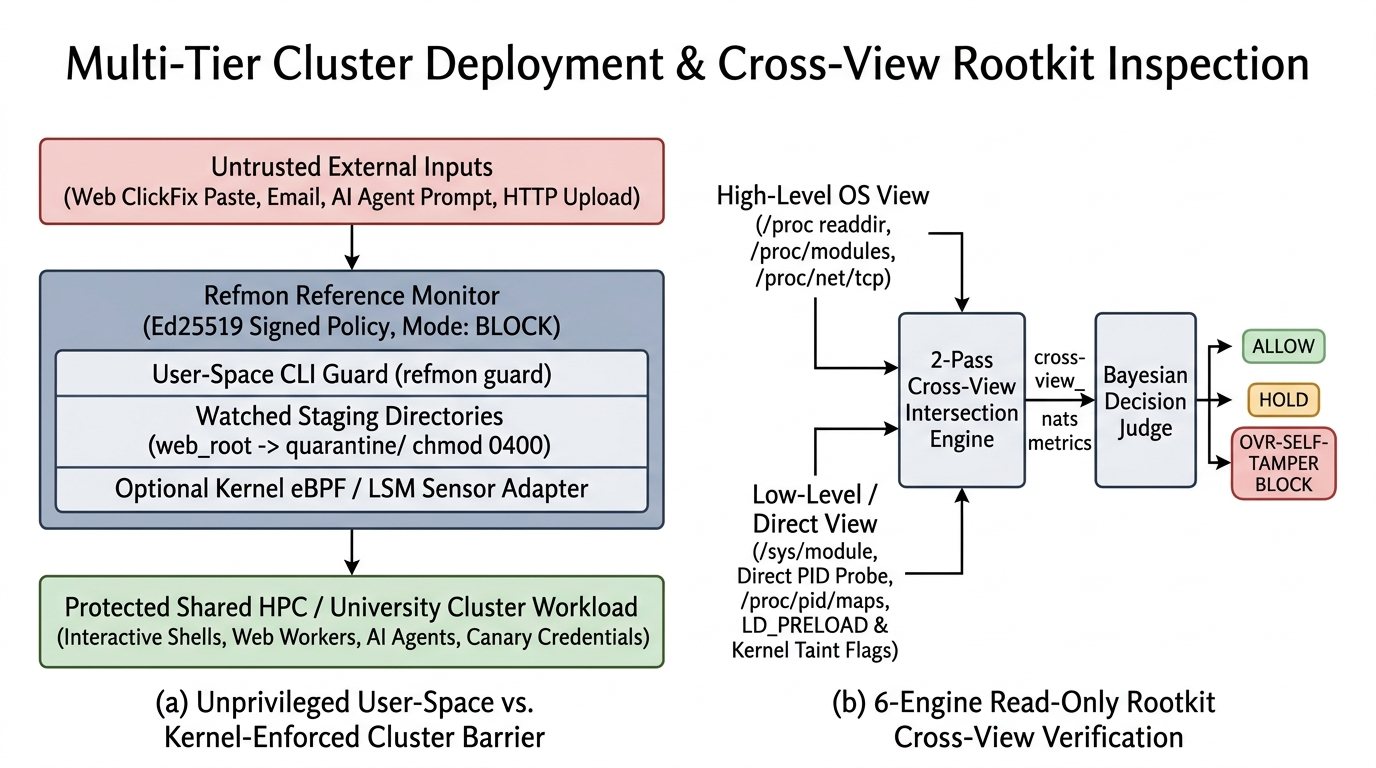
\includegraphics[width=0.95\textwidth]{figures/refmon_cluster_deployment.jpg}
  \caption{Multi-tier deployment architecture and host integrity verification: (a)~unprivileged user-space command barrier (\texttt{refmon guard}) and watched staging directories (\texttt{web\_root} $\to$ \texttt{quarantine/} mode \texttt{0400}) alongside optional kernel eBPF/LSM sensors; (b)~six-engine two-pass cross-view rootkit sensor feeding bounded log-odds into the Bayesian decision judge.}
  \label{fig:cluster_deployment}
\end{figure*}

Figure~\ref{fig:cluster_deployment} illustrates how Refmon protects shared Linux HPC nodes where researchers lack \texttt{root} privileges. The background service (\texttt{refmon serve}) verifies the Ed25519-signed policy, monitors user-space staging directories every $400$~ms, and provides a lightweight local telemetry interface. Because all local users on a shared multi-tenant cluster can connect to localhost network ports, every API call requires a per-daemon secret token stored in a private directory (\texttt{mode 0700}), and all requests with non-local HTTP \texttt{Host} headers are rejected to prevent DNS rebinding attacks.

Table~\ref{tab:live_suite} (Appendix~\ref{app:supplementary}) shows results from our live 16-scenario test suite ($16/16 = 100\%$ expected verdicts):
\begin{itemize}[leftmargin=1.3em,itemsep=1.5pt,topsep=2pt]
  \item \textbf{ClickFix Interception:} Pasted terminal attack commands are intercepted and halted prior to shell execution ($\texttt{executed=False}$).
  \item \textbf{Automated Quarantine:} Malicious PHP web shells dropped into staging directories are quarantined into read-only files (\texttt{mode 0400}) within $< 500$~ms.
  \item \textbf{Ransomware Suppression:} Sudden bursts of file modifications trigger automatic \texttt{mass\_change} blocks.
  \item \textbf{Benign Workload Freedom:} Legitimate operations (such as installing Python packages via PyPI or running local benchmarks) proceed with zero false alarms.
\end{itemize}
In host integrity scans, the rootkit engine suppresses benign GPU driver kernel taints ($L = -6.91 \mapsto \texttt{ALLOW}$), places unusual anonymous memory regions on hold ($L = -4.71 \mapsto \texttt{HOLD}$), and blocks preload implants, hidden kernel modules, and stealth processes ($L \ge -2.51 \mapsto \texttt{BLOCK}$).

\paragraph{Pre-Execution Command Intent Prediction.} To protect interactive terminals, Refmon inspects commands *before* the shell executes them. The barrier analyzes typed commands to predict the events they would produce, checking for hidden network tunnels (\texttt{socat}, netcat, reverse SSH shells), attempts to read sensitive credentials (\texttt{.aws}, \texttt{.kube}, private SSH keys), modifications to startup scripts or git hooks, and attempts to wipe shell history. To counter common shell obfuscation techniques, Refmon evaluates commands both as written and after stripping quotes, backslashes, and variable insertions (such as \texttt{\$\{IFS\}}). Table~\ref{tab:intent} (Appendix~\ref{app:supplementary}) summarizes this coverage across 69 diverse probe commands.

\subsection{Adversarial Privacy Audit and Test Suite Summary}
\label{sec:privacy_eval}

Running \texttt{refmon audit} executes an active red-team privacy audit across all generated verdicts, reports, stories, buffered events, learning proposals, and golden files:
\begin{itemize}[leftmargin=1.3em,itemsep=1pt,topsep=2pt]
  \item \textbf{Cleartext Leakage:} $264$ output artefacts scanned $\to$ \textbf{$0$ raw content findings}.
  \item \textbf{Dictionary HMAC Attack:} $349$ fingerprints attacked across $2,119$ common command/URL guesses without $K_{\text{dev}}$ $\to$ \textbf{$0$ reversals} (whereas a positive control given $K_{\text{dev}}$ reverses $6/6$, confirming attack-harness validity).
  \item \textbf{Four-Eyes Escrow:} $10$ single-approver re-identification attempts $\to$ \textbf{$0$ permitted}; dual-approver requests succeed with hash-chain integrity verified ($\texttt{audit chain intact = True}$).
  \item \textbf{Automated Verification:} Across unit, Hypothesis property-based, golden replay, variant-matrix, rootkit, command-intent, CLI, and live HTTP tests, over $1,860$ automated tests pass.
\end{itemize}

\clearpage
% ============================================================================
% 5. DISCUSSION
% ============================================================================
\section{Discussion}
\label{sec:discussion}
Attacks change payloads constantly, but what they do after gaining a foothold stays tied to OS rules: a web worker spawning a shell or dropping scripts will always break its role contract, no matter how clever the exploit. Refmon catches these actions by checking what happened instead of guessing what the payload looked like, while leaving ordinary developer commands alone. Fixing evidence monotonicity in \texttt{v1.3} and scoping trust to process lineage in \texttt{v2.0} closed edge-case leaks and cut false blocks to zero without widening permissions. Refmon keeps decisions deterministic rather than using reinforcement learning at runtime, avoiding reward poisoning and unexplainable black-box actions. Where gaps remain---such as out-of-band typed commands or slow leaks spread across hours---Refmon holds for human review rather than guessing, providing a reliable defense on shared nodes until kernel eBPF hooks can be deployed.

% ============================================================================
% 6. FUTURE WORK
% ============================================================================
\section{Future Work}
\label{sec:future}
We plan to hook Refmon directly into Linux \texttt{eBPF} LSM and \texttt{fanotify} for non-bypassable kernel-level mediation across all processes. We are also extending provenance tracking across multi-node Slurm and MPI batch jobs on shared clusters, tuning multi-day drift detectors for ultra-slow ransomware, and backing policy keys with TPM hardware roots of trust before running a longitudinal campus pilot.

% ============================================================================
% 7. CONCLUSION
% ============================================================================
\section{Conclusion}
\label{sec:conclusion}
Refmon demonstrates that tracking behavioral consequences rather than exploit payloads provides a reliable, privacy-preserving defense against zero-day exploits, ClickFix lures, and stealth rootkits. Evaluated across 46 golden scenarios, 886 mutation variants, and a live cluster barrier suite, Refmon achieves 100\% golden accuracy and 98.4\% attack containment with zero false blocks on benign workloads. Its mathematically verified monotonicity, minimal Bayes risk, and in-memory privacy boundary make it a practical, robust security foundation for shared computing clusters.

% ============================================================================
% 8. AI DISCLOSURE
% ============================================================================
\section{AI Disclosure}
\label{sec:ai_disclosure}
Generative AI assistants (Claude Code and Antigravity) were used under human supervision to help write code, generate test suites, render diagrams, and typeset this document from a human-written specification. No AI or machine-learning model runs inside the Refmon decision engine; every runtime verdict is a deterministic calculation governed by signed policies and proven mathematics. All signal weights were frozen prior to evaluation, mutation streams used pre-registered random seeds, policy keys remained strictly human-held, and all empirical claims were validated by executable test suites.

% ============================================================================
% REFERENCES (SINGLE COLUMN)
% ============================================================================
\clearpage
\onecolumn

\begin{thebibliography}{99}\small\raggedright

\bibitem{anderson1972computer}
J.~P. Anderson, ``Computer security technology planning study,'' Electronic Systems Division, Air Force Systems Command, Tech. Rep. ESD-TR-73-51, Vol.~II, Oct. 1972.

\bibitem{denning1976lattice}
D.~E. Denning, ``A lattice model of secure information flow,'' \emph{Communications of the ACM}, vol.~19, no.~5, pp.~236--243, May 1976.

\bibitem{wald1945sequential}
A.~Wald, ``Sequential tests of statistical hypotheses,'' \emph{The Annals of Mathematical Statistics}, vol.~16, no.~2, pp.~117--186, Jun. 1945.

\bibitem{page1954continuous}
E.~S. Page, ``Continuous inspection schemes,'' \emph{Biometrika}, vol.~41, no.~1/2, pp.~100--115, Jun. 1954.

\bibitem{lorden1971procedures}
G.~Lorden, ``Procedures for reacting to a change in distribution,'' \emph{The Annals of Mathematical Statistics}, vol.~42, no.~6, pp.~1897--1908, Dec. 1971.

\bibitem{good1953population}
I.~J. Good, ``The population frequencies of species and the estimation of population parameters,'' \emph{Biometrika}, vol.~40, no.~3/4, pp.~237--264, Dec. 1953.

\bibitem{pearl1988probabilistic}
J.~Pearl, \emph{Probabilistic Reasoning in Intelligent Systems: Networks of Plausible Inference}. San Mateo, CA: Morgan Kaufmann, 1988.

\bibitem{bloom1970space}
B.~H. Bloom, ``Space/time trade-offs in hash coding with allowable errors,'' \emph{Communications of the ACM}, vol.~13, no.~7, pp.~422--426, Jul. 1970.

\bibitem{bellare1996keying}
M.~Bellare, R.~Canetti, and H.~Krawczyk, ``Keying hash functions for message authentication,'' in \emph{Advances in Cryptology --- CRYPTO '96}, LNCS vol.~1109, pp.~1--15, Springer, 1996.

\bibitem{bernstein2012high}
D.~J. Bernstein, N.~Duif, T.~Lange, P.~Schwabe, and B.-Y. Yang, ``High-speed high-security signatures,'' \emph{Journal of Cryptographic Engineering}, vol.~2, no.~2, pp.~77--89, Sep. 2012.

\bibitem{dwork2006calibrating}
C.~Dwork, F.~McSherry, K.~Nissim, and A.~Smith, ``Calibrating noise to sensitivity in private data analysis,'' in \emph{Proc. Theory of Cryptography Conf. (TCC)}, LNCS vol.~3876, pp.~265--284, Springer, 2006.

\bibitem{sweeney2002kanonymity}
L.~Sweeney, ``$k$-anonymity: A model for protecting privacy,'' \emph{Int. J. Uncertainty, Fuzziness and Knowledge-Based Systems}, vol.~10, no.~5, pp.~557--570, Oct. 2002.

\bibitem{newsome2005dynamic}
J.~Newsome and D.~X. Song, ``Dynamic taint analysis for automatic detection, analysis, and signature generation of exploits on commodity software,'' in \emph{Proc. NDSS}, Feb. 2005.

\bibitem{pasquier2017practical}
T.~Pasquier, X.~Han, M.~Goldstein, T.~Moyer, D.~Eyers, M.~Seltzer, and J.~Bacon, ``Practical whole-system provenance capture,'' in \emph{Proc. ACM SoCC}, pp.~405--418, Sep. 2017.

\bibitem{hossain2017sleuth}
M.~N. Hossain, S.~M. Milajerdi, J.~Wang, B.~Eshete, R.~Gjomemo, R.~Sekar, S.~Stolper, and V.~N. Venkatakrishnan, ``SLEUTH: Real-time attack scenario reconstruction from COTS audit data,'' in \emph{Proc. USENIX Security Symp.}, pp.~487--504, Aug. 2017.

\bibitem{milajerdi2019holmes}
S.~M. Milajerdi, R.~Gjomemo, B.~Eshete, R.~Sekar, and V.~N. Venkatakrishnan, ``HOLMES: Real-time APT detection through correlation of suspicious information flows,'' in \emph{Proc. IEEE Symp. Security and Privacy (S\&P)}, pp.~1137--1152, May 2019.

\bibitem{han2020unicorn}
X.~Han, T.~Pasquier, A.~Bates, J.~Mickens, and M.~Seltzer, ``UNICORN: Runtime provenance-based detector for advanced persistent threats,'' in \emph{Proc. NDSS}, Feb. 2020.

\bibitem{smalley2001implementing}
S.~Smalley, C.~Vance, and W.~Salamon, ``Implementing SELinux as a Linux Security Module,'' NAI Labs Report \#01-043, Dec. 2001.

\bibitem{bauer2006paranoid}
M.~Bauer, ``Paranoid penguin: An introduction to Novell AppArmor,'' \emph{Linux Journal}, vol.~2006, no.~148, p.~13, Aug. 2006.

\bibitem{corbet2012seccomp}
J.~Corbet, ``Seccomp filter (Mode 2 BPF syscall filtering),'' Linux Kernel Documentation (\texttt{Documentation/userspace-api/seccomp\_filter.rst}), 2012.

\bibitem{wang2005strider}
Y.-M. Wang, D.~Beck, B.~Vo, R.~Roussev, and C.~Verbowski, ``Detecting stealth software with Strider GhostBuster,'' in \emph{Proc. IEEE/IFIP Int. Conf. Dependable Systems and Networks (DSN)}, pp.~368--377, Jun. 2005.

\bibitem{garfinkel2003virtual}
T.~Garfinkel and M.~Rosenblum, ``A virtual machine introspection based architecture for intrusion detection,'' in \emph{Proc. NDSS}, pp.~191--206, Feb. 2003.

\bibitem{jung2004fast}
J.~Jung, V.~Paxson, A.~W. Berger, and H.~Balakrishnan, ``Fast portscan detection using sequential hypothesis testing,'' in \emph{Proc. IEEE Symp. Security and Privacy (S\&P)}, pp.~211--225, May 2004.

\bibitem{greshake2023not}
K.~Greshake, S.~Abdelnabi, S.~Mishra, C.~Endres, T.~Holz, and M.~Fritz, ``Not what you've signed up for: Compromising real-world LLM-integrated applications with indirect prompt injection,'' in \emph{Proc. ACM AISec Workshop}, pp.~79--90, Nov. 2023.

\bibitem{mitre2024attack}
MITRE Corporation, ``MITRE ATT\&CK Enterprise Matrix (T1204.004 User Execution: Malicious Copy and Paste),'' Technical Knowledge Base, 2024--2026.

\bibitem{wilson1927probable}
E.~B. Wilson, ``Probable inference, the law of succession, and statistical inference,'' \emph{Journal of the American Statistical Association}, vol.~22, no.~158, pp.~209--212, Jun. 1927.

\bibitem{mcnemar1947note}
Q.~McNemar, ``Note on the sampling error of the difference between correlated proportions or percentages,'' \emph{Psychometrika}, vol.~12, no.~2, pp.~153--157, Jun. 1947.

\end{thebibliography}

% ============================================================================
% APPENDICES: COMPLETE MATHEMATICAL PROOFS
% ============================================================================
\clearpage
\appendix

\section{Supplementary Architecture, Implementation, and Verification Data}
\label{app:supplementary}

This appendix provides the end-to-end pipeline architecture figure, the frozen evidence calculus weights, the user-space command barrier loop, and the complete verification tables referenced in the main text.

\begin{figure}[!htbp]
  \centering
  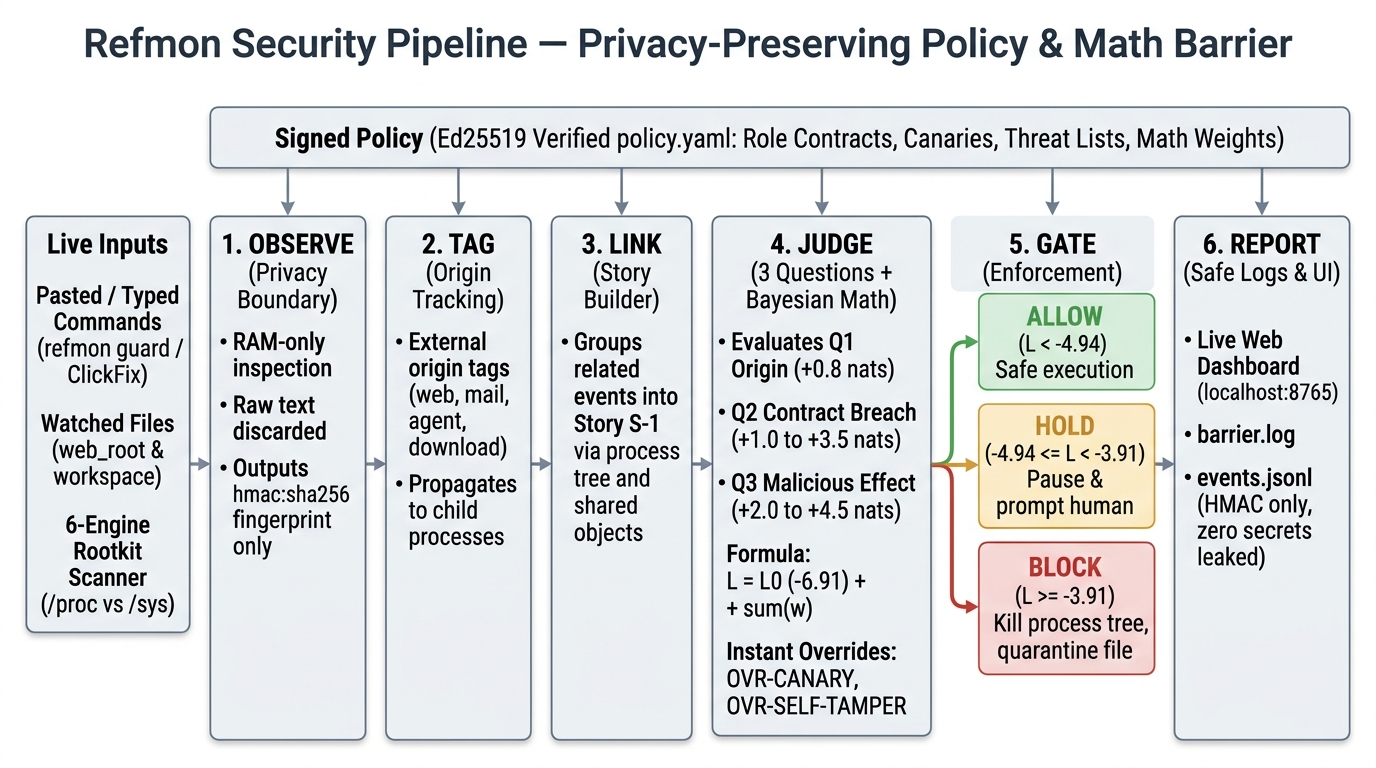
\includegraphics[width=0.92\textwidth]{figures/refmon_pipeline.jpg}
  \caption{Architectural overview of the six-stage Refmon Security Pipeline. Raw inputs are processed strictly in volatile memory during Stage~1 (\texttt{Observe}) and reduced to keyed \texttt{hmac:sha256} digests before reaching provenance tagging, story linking, Bayesian judging, containment gating, and privacy reporting.}
  \label{fig:pipeline_img}
\end{figure}

\begin{table}[!htbp]
  \centering
  \caption{Frozen \texttt{v1.3} Policy Signal Weights ($w_j$ in nats) and Cost Parameters ($\pi = 0.001$, $C_{\text{miss}}=1000$, $C_{\text{fb}}=20$, $C_{\text{hold}}=5$, $h=0.7$).}
  \label{tab:weights}
  \small
  \begin{tabular}{@{}llrlr@{}}
    \toprule
    \textbf{Axis} & \textbf{Signal Name} & \textbf{$w_j$} & \textbf{Signal Name} & \textbf{$w_j$} \\
    \midrule
    Origin   & \texttt{origin\_external} & $0.8$ & --- & --- \\
    \midrule
    Contract & \texttt{external\_exec} & $1.0$ & \texttt{write\_other} & $1.0$ \\
             & \texttt{unsigned\_launch} & $1.5$ & \texttt{surprisal} & $2.0$ \\
             & \texttt{universal\_violation} & $2.0$ & \texttt{exec\_violation} & $2.5$ \\
             & \texttt{connect\_violation} & $2.5$ & \texttt{asset\_violation} & $2.5$ \\
             & \texttt{web\_worker\_exec} & $3.0$ & \texttt{write\_executable} & $3.5$ \\
             & \texttt{persist\_violation} & $3.5$ & \texttt{privilege\_violation} & $3.5$ \\
    \midrule
    Effect   & \texttt{asset\_access} & $1.5$ & \texttt{response\_anomaly} & $1.5$ \\
             & \texttt{hide} & $2.0$ & \texttt{fetch} & $2.5$ \\
             & \texttt{persist} & $2.5$ & \texttt{exfil} & $2.5$ \\
             & \texttt{escalate} & $2.5$ & \texttt{mass\_change} & $2.5$ \\
             & \texttt{tamper} & $3.0$ & \texttt{lateral} & $3.5$ \\
             & \texttt{credential} & $3.5$ & \texttt{resp\_anom\_repeated} & $3.5$ \\
             & \texttt{threat\_list\_hit} & $4.5$ & --- & --- \\
    \bottomrule
  \end{tabular}
\end{table}

\begin{lstlisting}[language=Python,style=refmoncode,caption={Core unprivileged user-space command barrier loop (excerpted from \texttt{src/refmon/live.py}).},label={lst:barrier}]
story_id, j = self._feed_raw_events(raw_events)  # Observe -> Tag -> Link -> Judge -> Gate
lo = float(j.log_odds if j.log_odds is not None else 0.0)
blocked_by_barrier = (
    self.policy.mode is Mode.BLOCK
    and j.decision in (Decision.BLOCK, Decision.HOLD)
)
if execute and not blocked_by_barrier and j.decision is Decision.ALLOW:
    proc = subprocess.run(cmd, shell=True, cwd=str(self.workspace_dir),
                          capture_output=True, text=True, timeout=5.0, check=False)
\end{lstlisting}

\begin{table}[!htbp]
  \centering
  \caption{Command-Barrier Probes Typed Locally (\texttt{mode=block}). Bold: the held-out measurement.}
  \label{tab:intent}
  \small
  \begin{tabular}{@{}lrrr@{}}
    \toprule
    \textbf{Probe set} & \textbf{\texttt{v1.7}} & \textbf{\texttt{v2.0} first run} & \textbf{\texttt{v2.0} now} \\
    \midrule
    23 attacker behaviours (\texttt{test\_intent.py}) & $23/23$ & $23/23$ & $23/23$ \\
    20 evasions, written before A67 & $11/20$ & $20/20$ & $20/20$ \\
    20 attacks, held out & $13/20$ & $\mathbf{15/20}$ & $20/20$ \\
    \midrule
    23 + 14 benign look-alikes (false alarms) & $1$ & $0$ & $0$ \\
    15 benign, held out (false alarms) & $1$ & $\mathbf{1}$ & $0$ \\
    \bottomrule
  \end{tabular}
\end{table}

\begin{table}[!htbp]
  \centering
  \caption{Live Barrier 16-Scenario Verification Suite (\texttt{mode=block}).}
  \label{tab:live_suite}
  \small
  \begin{tabular}{@{}llrrl@{}}
    \toprule
    \textbf{Scenario Type} & \textbf{Origin / Role} & \textbf{Q-Fails} & \textbf{$L$ (nats)} & \textbf{Verdict} \\
    \midrule
    ClickFix Paste (\texttt{curl|sh}) & \texttt{web} / \texttt{shell} & $3/3$ & $-0.61$ & \texttt{BLOCK} \\
    Obfuscated Base64 Mail & \texttt{mail} / \texttt{shell} & $3/3$ & $-3.11$ & \texttt{BLOCK} \\
    AI Prompt-Injection Abuse & \texttt{agent\_in} / \texttt{agent} & $3/3$ & $-0.11$ & \texttt{BLOCK} \\
    Protected Credential Theft & \texttt{mail} / \texttt{shell} & OVR & $-1.61$ & \texttt{BLOCK} \\
    Server Web Worker RCE & \texttt{req\_in} / \texttt{web} & $3/3$ & $-0.61$ & \texttt{BLOCK} \\
    Web Shell Drop (\texttt{.php}) & \texttt{req\_in} / \texttt{web} & $3/3$ & $-0.11$ & \texttt{BLOCK+QUAR} \\
    Ransomware 55-File Burst & local / \texttt{shell} & $2/3$ & $-2.41$ & \texttt{BLOCK} \\
    Decoy Canary Credential & \texttt{web} / \texttt{shell} & OVR & $-1.61$ & \texttt{BLOCK} \\
    SUID / \texttt{sudo} Escalation & \texttt{dl} / \texttt{shell} & $3/3$ & $-2.61$ & \texttt{BLOCK} \\
    Crontab / \texttt{.bashrc} Persist & \texttt{web} / \texttt{shell} & $3/3$ & $-2.61$ & \texttt{BLOCK} \\
    Security Tamper (\texttt{pkill}) & local / \texttt{shell} & OVR & $-1.91$ & \texttt{BLOCK} \\
    Supply-Chain Post-Install & \texttt{pkg} / \texttt{installer} & $3/3$ & $+1.89$ & \texttt{BLOCK} \\
    \midrule
    Unverified Mirror Fetch & local / \texttt{shell} & $1/3$ & $-4.41$ & \texttt{HOLD} \\
    \midrule
    Benign Local \texttt{ls -la} & local / \texttt{shell} & $0/3$ & $-6.91$ & \texttt{ALLOW} \\
    Benign Pasted \texttt{echo} & \texttt{web} / \texttt{shell} & $2/3$ & $-5.11$ & \texttt{ALLOW} \\
    Trusted PyPI Download & \texttt{dl} / \texttt{installer} & OVR & $-6.91$ & \texttt{ALLOW} \\
    \bottomrule
  \end{tabular}
\end{table}

\section{Proofs of Provenance Decay and Noisy-OR Fusion}
\label{app:decay}

\begin{proposition}[Monotonicity and Invariance of Label Decay]
\label{prop:decay}
Let $s_\ell(t) = s_0 \cdot 2^{-(t - t_0)/T_{1/2}}$ for $s_0 \in [0, 1]$, $T_{1/2} > 0$, and $t \ge t_0$. Then:
\begin{enumerate}[leftmargin=1.5em,itemsep=1pt,topsep=2pt]
  \item $s_\ell(t) \in [0, s_0] \subseteq [0, 1]$ for all $t \ge t_0$;
  \item $s_\ell(t)$ is strictly decreasing in $t$ whenever $s_0 > 0$, with $s_\ell(t_0 + k T_{1/2}) = 2^{-k} s_0$;
  \item Under edge attenuation $a_e \in (0, 1]$, any $d$-hop causal path $p = (e_1, \dots, e_d)$ satisfies $s_{\text{leaf}}(t) = s_0 \big(\prod_{r=1}^{d} a_{e_r}\big) 2^{-\Delta t / T_{1/2}} \le s_\ell(t)$.
\end{enumerate}
\end{proposition}
\begin{proof}
Since $T_{1/2} > 0$ and $\Delta t = t - t_0 \ge 0$, we have $-\Delta t / T_{1/2} \le 0$, so $0 < 2^{-\Delta t / T_{1/2}} \le 1$, proving $0 \le s_\ell(t) \le s_0 \le 1$. Differentiating with respect to $t$ yields
\[
  \frac{\mathrm{d}s_\ell(t)}{\mathrm{d}t} = -\frac{\ln 2}{T_{1/2}}\, s_0 \, 2^{-(t - t_0)/T_{1/2}} < 0 \quad (\forall s_0 > 0),
\]
establishing strict temporal monotonicity, and direct substitution of $\Delta t = k T_{1/2}$ gives $s_\ell(t_0 + k T_{1/2}) = 2^{-k}s_0$. Finally, because $a_{e_r} \in (0, 1]$ for every edge $e_r$, induction over path length $d$ yields $0 < \prod_{r=1}^{d} a_{e_r} \le 1$, whence $s_{\text{leaf}}(t) \le s_\ell(t)$.
\end{proof}

\begin{theorem}[Algebraic and Dominance Properties of Noisy-OR]
\label{thm:noisyor}
For any finite multiset of label strengths $\mathbf{s} = (s_1, \dots, s_m) \in [0, 1]^m$, define $\operatorname{NOR}(\mathbf{s}) = 1 - \prod_{i=1}^{m}(1 - s_i)$ (with empty product $1$). Then:
\begin{enumerate}[leftmargin=1.5em,itemsep=1pt,topsep=2pt]
  \item \textbf{Range closure:} $\operatorname{NOR}(\mathbf{s}) \in [0, 1]$;
  \item \textbf{Dominance:} $\max_{1 \le i \le m} s_i \le \operatorname{NOR}(\mathbf{s}) \le \min\!\big(1, \sum_{i=1}^{m} s_i\big)$;
  \item \textbf{Commutative monoid:} $\operatorname{NOR}$ is symmetric, associative under binary composition $x \oplus y = 1 - (1-x)(1-y) = x + y - xy$, has identity element $0$, and absorbing element $1$;
  \item \textbf{Coordinate-wise monotonicity:} If $s_i \le s'_i$ for all $i$, then $\operatorname{NOR}(\mathbf{s}) \le \operatorname{NOR}(\mathbf{s}')$.
\end{enumerate}
\end{theorem}
\begin{proof}
(1) Since $s_i \in [0, 1]$, each factor satisfies $1 - s_i \in [0, 1]$, so $P = \prod_{i=1}^{m}(1 - s_i) \in [0, 1]$ and $1 - P \in [0, 1]$.

(2) Fix an arbitrary index $k \in \{1, \dots, m\}$. Because $\prod_{i \neq k}(1 - s_i) \le 1$ and $1 - s_k \ge 0$, we obtain
\begin{align*}
  \prod_{i=1}^{m}(1 - s_i) &= (1 - s_k)\prod_{i \neq k}(1 - s_i) \le 1 - s_k\\
  &\implies \operatorname{NOR}(\mathbf{s}) \ge s_k.
\end{align*}
Taking the maximum over $k$ yields $\operatorname{NOR}(\mathbf{s}) \ge \max_i s_i$. For the upper bound, induction on $m$ using Weierstrass's inequality $\prod_{i=1}^{m}(1 - s_i) \ge 1 - \sum_{i=1}^{m} s_i$ gives $\operatorname{NOR}(\mathbf{s}) \le \sum_{i=1}^{m} s_i$, and combining with (1) gives $\min(1, \sum_i s_i)$.

(3) Symmetry follows from commutativity of real multiplication. For associativity, $(x \oplus y) \oplus z = 1 - (1 - [1 - (1-x)(1-y)])(1-z) = 1 - (1-x)(1-y)(1-z) = x \oplus (y \oplus z)$. Moreover, $x \oplus 0 = 1 - (1-x)\cdot 1 = x$ and $x \oplus 1 = 1 - (1-x)\cdot 0 = 1$.

(4) If $s_i \le s'_i$, then $0 \le 1 - s'_i \le 1 - s_i$ for each $i$, so $\prod_{i=1}^{m}(1 - s'_i) \le \prod_{i=1}^{m}(1 - s_i)$, whence $\operatorname{NOR}(\mathbf{s}) \le \operatorname{NOR}(\mathbf{s}')$.
\end{proof}

% ============================================================================
\section{Derivation of Bayes-Optimal Thresholds and Contract Gate}
\label{app:bayes}

\begin{theorem}[Bayes Minimal-Risk Log-Odds Thresholds]
\label{thm:bayes_thresholds}
Let $Y \in \{0, 1\}$ denote whether a story $S$ is benign ($Y=0$) or an attack ($Y=1$), and let $p = \mathbb{P}(Y = 1 \mid S) = (1 + e^{-L})^{-1}$ be the posterior attack probability corresponding to log-odds $L = \ln\frac{p}{1-p}$. Suppose:
\begin{itemize}[leftmargin=1.4em,itemsep=1pt,topsep=2pt]
  \item Action $a_{\text{allow}}$ incurs loss $C_{\text{miss}} > 0$ if $Y=1$ and $0$ if $Y=0$;
  \item Action $a_{\text{block}}$ incurs loss $0$ if $Y=1$ and $C_{\text{fb}} > 0$ if $Y=0$;
  \item Action $a_{\text{hold}}$ incurs human-review cost $C_{\text{hold}} > 0$ if $Y=0$, and catches a true attack ($Y=1$) with probability $h \in (0, 1]$ (leaving residual miss cost $(1 - h)C_{\text{miss}}$; when $C_{\text{hold}} \ll C_{\text{miss}}$ we neglect the $O(C_{\text{hold}})$ operational overhead under $Y=1$).
\end{itemize}
Then:
\begin{enumerate}[leftmargin=1.5em,itemsep=1.5pt,topsep=2pt]
  \item Pairwise preference $R(a_{\text{block}} \mid S) \le R(a_{\text{allow}} \mid S)$ holds iff
  \[
    L \ge \tau_{\text{block}} \triangleq \ln\frac{C_{\text{fb}}}{C_{\text{miss}}};
  \]
  \item Pairwise preference $R(a_{\text{hold}} \mid S) \le R(a_{\text{allow}} \mid S)$ holds iff
  \[
    L \ge \tau_{\text{hold}} \triangleq \ln\frac{C_{\text{hold}}}{h \cdot C_{\text{miss}}};
  \]
  \item A non-empty \texttt{HOLD} interval $[\tau_{\text{hold}}, \tau_{\text{block}})$ exists iff $C_{\text{hold}} < h \cdot C_{\text{fb}}$.
\end{enumerate}
\end{theorem}
\begin{proof}
The conditional Bayes risks of the three actions given posterior $p \in (0, 1)$ are:
\begin{align*}
  R(a_{\text{allow}} \mid S) &= p \, C_{\text{miss}},\\
  R(a_{\text{block}} \mid S) &= (1 - p) \, C_{\text{fb}},\\
  R(a_{\text{hold}} \mid S)  &= p (1 - h) C_{\text{miss}} + (1 - p) C_{\text{hold}}.
\end{align*}
For (1), $R(a_{\text{block}} \mid S) \le R(a_{\text{allow}} \mid S)$ iff $(1 - p) C_{\text{fb}} \le p \, C_{\text{miss}}$, which rearranges to
\[
  \frac{p}{1 - p} \ge \frac{C_{\text{fb}}}{C_{\text{miss}}}
  \iff L = \ln\frac{p}{1 - p} \ge \ln\frac{C_{\text{fb}}}{C_{\text{miss}}} = \tau_{\text{block}}.
\]
For (2), $R(a_{\text{hold}} \mid S) \le R(a_{\text{allow}} \mid S)$ iff
\begin{align*}
  p(1 - h)C_{\text{miss}} + (1 - p)C_{\text{hold}} &\le p \, C_{\text{miss}}\\
  \iff (1 - p)C_{\text{hold}} &\le p \, h \, C_{\text{miss}}.
\end{align*}
Dividing by $(1 - p) h C_{\text{miss}} > 0$ and taking natural logarithms yields
\[
  \frac{p}{1 - p} \ge \frac{C_{\text{hold}}}{h \cdot C_{\text{miss}}}
  \iff L \ge \ln\frac{C_{\text{hold}}}{h \cdot C_{\text{miss}}} = \tau_{\text{hold}}.
\]
For (3), by strict monotonicity of $\ln(\cdot)$, $\tau_{\text{hold}} < \tau_{\text{block}} \iff \frac{C_{\text{hold}}}{h C_{\text{miss}}} < \frac{C_{\text{fb}}}{C_{\text{miss}}} \iff C_{\text{hold}} < h \, C_{\text{fb}}$. Substituting Refmon's default policy costs ($C_{\text{hold}} = 5$, $h = 0.7$, $C_{\text{fb}} = 20$) gives $5 < 14$, yielding $\tau_{\text{hold}} = \ln(5/700) = -4.9416 < \tau_{\text{block}} = \ln(20/1000) = -3.9120$.
\end{proof}

\begin{corollary}[Sensitivity Directionality]
$\partial \tau_{\text{block}} / \partial C_{\text{fb}} = 1/C_{\text{fb}} > 0$, $\partial \tau_{\text{block}} / \partial C_{\text{miss}} = -1/C_{\text{miss}} < 0$, and $\partial \tau_{\text{hold}} / \partial h = -1/h < 0$. Thus raising false-block penalties raises the evidence bar for blocking, whereas raising missed-attack cost lowers both thresholds monotonically.
\end{corollary}

% ============================================================================
\section{Proof of Posterior Monotonicity in \texttt{v1.3} (Resolution of F8)}
\label{app:monotone}

\begin{theorem}[Monotonicity of \texttt{v1.3} Calculus vs.\ Non-Monotonicity of \texttt{v1.2}]
\label{thm:monotone}
Fix a story $S$ with non-empty Contract or Effect signals having positive max weights $W_C = \max_{j \in \mathcal{S}_C} w_j > 0$ and $W_E = \max_{k \in \mathcal{S}_E} w_k \ge 0$, origin weight $w_{\text{ori}} \ge 0$, and origin threshold $\theta \in (0, 1)$.
\begin{enumerate}[leftmargin=1.5em,itemsep=1.5pt,topsep=2pt]
  \item Under the legacy \texttt{v1.2} rule $L_{\text{v1.2}}(s) = L_0 + w_{\text{ori}} s \mathbf{1}[s \ge \theta] + \big(s \mathbf{1}[s \ge \theta] + \mathbf{1}[s < \theta]\big)(W_C + W_E)$, $L_{\text{v1.2}}(s)$ is \textbf{not} non-decreasing on $[0, 1]$ whenever $W_C + W_E > \frac{\theta}{1 - \theta} w_{\text{ori}}$.
  \item Under the \texttt{v1.3} rule $L_{\text{v1.3}}(s) = L_0 + w_{\text{ori}} s \mathbf{1}[s \ge \theta] + W_C + W_E$, $L_{\text{v1.3}}(s)$ is monotonically non-decreasing over all $s \in [0, 1]$ and under arbitrary signal additions with $w_j \ge 0$.
\end{enumerate}
\end{theorem}
\begin{proof}
(1) Evaluate the left and right limits of $L_{\text{v1.2}}(s)$ at $s = \theta$:
\begin{align*}
  \lim_{s \uparrow \theta} L_{\text{v1.2}}(s) &= L_0 + W_C + W_E,\\
  L_{\text{v1.2}}(\theta) &= L_0 + \theta w_{\text{ori}} + \theta(W_C + W_E).
\end{align*}
Hence $L_{\text{v1.2}}(\theta) - \lim_{s \uparrow \theta} L_{\text{v1.2}}(s) = \theta w_{\text{ori}} - (1 - \theta)(W_C + W_E)$. For Refmon's defaults ($\theta = 0.5$, $w_{\text{ori}} = 0.8$), whenever $W_C + W_E > 0.8$ (which holds for \emph{every} Contract + Effect pair in Table~\ref{tab:weights}, e.g., $W_C + W_E = 1.0 + 2.5 = 3.5$), we have $L_{\text{v1.2}}(0.5) - L_{\text{v1.2}}(0.499) = 0.4 - 1.75 = -1.35 < 0$, proving a downward jump where stronger provenance produced weaker evidence.

(2) In \texttt{v1.3}, write $g(s) = w_{\text{ori}} s \mathbf{1}[s \ge \theta]$. For $0 \le s_1 \le s_2 < \theta$, $g(s_1) = g(s_2) = 0$. For $0 \le s_1 < \theta \le s_2 \le 1$, since $w_{\text{ori}} \ge 0$ and $s_2 \ge \theta > 0$, $g(s_1) = 0 \le w_{\text{ori}} s_2 = g(s_2)$. For $\theta \le s_1 \le s_2 \le 1$, $g(s_2) - g(s_1) = w_{\text{ori}}(s_2 - s_1) \ge 0$. Since $W_C$ and $W_E$ are independent of $s$ (apart from D23's indicator $\mathbf{1}[s \ge \theta]$ which only \emph{adds} positive allowed-effect weights when $s$ crosses $\theta$), $L_{\text{v1.3}}(s_1) \le L_{\text{v1.3}}(s_2)$ for all $0 \le s_1 \le s_2 \le 1$. Furthermore, adding any signal $j^*$ with $w_{j^*} \ge 0$ to question set $\mathcal{S}_q$ satisfies $\max_{j \in \mathcal{S}_q \cup \{j^*\}} w_j s_j \ge \max_{j \in \mathcal{S}_q} w_j s_j$, so $L_{\text{v1.3}}$ never decreases when evidence is added.
\end{proof}

% ============================================================================
\section{Proofs of Laplace Surprisal and Good-Turing Unseen Mass}
\label{app:rarity}

\begin{proposition}[Properness and Surprisal Bounds of Laplace Role Model]
Let $n_1, \dots, n_K \ge 1$ be observed counts summing to $N = \sum_{e=1}^{K} n_e$, and define $\hat{p}(e) = \frac{n_e + \alpha}{N + \alpha(K + 1)}$ for $e \in \{1, \dots, K\}$ and $\hat{p}(\text{unseen}) = \frac{\alpha}{N + \alpha(K + 1)}$ with $\alpha > 0$. Then $\hat{p}$ is a valid probability distribution on $\{1, \dots, K, \text{unseen}\}$, and unseen-event surprisal satisfies $I(\text{unseen}) = \log_2\!\big(\frac{N}{\alpha} + K + 1\big)$.
\end{proposition}
\begin{proof}
Every probability is strictly positive since $n_e \ge 0$ and $\alpha > 0$. Summing over all $K + 1$ outcomes gives
\begin{align*}
  &\sum_{e=1}^{K} \frac{n_e + \alpha}{N + \alpha(K + 1)} + \frac{\alpha}{N + \alpha(K + 1)}\\
  &\quad = \frac{\sum_{e=1}^{K} n_e + K\alpha + \alpha}{N + \alpha(K + 1)} = \frac{N + \alpha(K + 1)}{N + \alpha(K + 1)} = 1.
\end{align*}
Taking $-\log_2 \hat{p}(\text{unseen})$ yields $\log_2((N + \alpha(K+1))/\alpha) = \log_2(N/\alpha + K + 1)$. In particular, for $\alpha = 1$, $I(\text{unseen}) \ge 12$~bits requires $N + K + 1 \ge 2^{12} = 4096$, automatically preventing surprisal false alarms on small samples even before the Good-Turing check.
\end{proof}

\begin{theorem}[Unbiasedness of Good-Turing Unseen Probability Estimator~\cite{good1953population}]
\label{thm:goodturing}
Suppose $N$ i.i.d.\ events are drawn from an unknown discrete distribution $\{p_e\}_{e \in \mathcal{U}}$ over a countable alphabet $\mathcal{U}$. Let $N_e$ be the count of kind $e$ in the first $N$ draws, $U_N = \sum_{e \in \mathcal{U}} p_e \mathbf{1}[N_e = 0]$ be the true random probability mass of kinds unseen in $N$ draws, and $N_1^{(N+1)} = \sum_{e \in \mathcal{U}} \mathbf{1}[N'_e = 1]$ be the number of singletons in a sample of size $N + 1$. Then:
\[
  \mathbb{E}[U_N] = \frac{\mathbb{E}\big[N_1^{(N+1)}\big]}{N + 1} \approx \frac{\mathbb{E}[N_1^{(N)}]}{N}.
\]
\end{theorem}
\begin{proof}
By linearity of expectation and $N_e \sim \operatorname{Binomial}(N, p_e)$,
\[
  \mathbb{E}[U_N] = \sum_{e \in \mathcal{U}} p_e \mathbb{P}(N_e = 0) = \sum_{e \in \mathcal{U}} p_e (1 - p_e)^N.
\]
Conversely, in $N + 1$ i.i.d.\ draws, $\mathbb{P}(N'_e = 1) = (N + 1) p_e (1 - p_e)^N$. Summing over $e \in \mathcal{U}$ and dividing by $N + 1$ gives
\begin{align*}
  \frac{\mathbb{E}\big[N_1^{(N+1)}\big]}{N + 1} &= \frac{1}{N + 1}\sum_{e \in \mathcal{U}} (N + 1) p_e (1 - p_e)^N\\
  &= \sum_{e \in \mathcal{U}} p_e (1 - p_e)^N = \mathbb{E}[U_N].
\end{align*}
For $N \gg 1$, replacing $N+1$ by $N$ yields $\hat{p}_{\text{unseen}} = N_1 / N$ with $O(1/N)$ bias.
\end{proof}

% ============================================================================
\section{Proofs of Statistical Rate and CUSUM Drift Properties}
\label{app:stats}

\begin{proposition}[Numerical Exactness of Upper-Tail Poisson Recurrence]
For $X \sim \operatorname{Poisson}(\lambda)$ with $\lambda > 0$ and integer $k \ge 1$, the upper tail $T(k, \lambda) = \sum_{i=k}^{\infty} t_i$ with $t_k = \exp(-\lambda + k \ln \lambda - \ln \Gamma(k + 1))$ and recurrence $t_{i+1} = t_i \cdot \frac{\lambda}{i + 1}$ converges strictly monotonically for $i \ge \lceil \lambda \rceil$ with relative truncation error below machine epsilon $\varepsilon_{\text{mach}}$ once $t_i \le \varepsilon_{\text{mach}} \sum_{j=k}^{i} t_j$.
\end{proposition}
\begin{proof}
Computing $\ln t_k$ via $\operatorname{lgamma}(k + 1) = \ln(k!)$ avoids catastrophic cancellation in $1 - \sum_{i=0}^{k-1} t_i$ when $T(k, \lambda) \approx 10^{-12} \ll \varepsilon_{\text{mach}} \approx 2.22 \times 10^{-16}$ (where complement subtraction returns $0.0$). For all $i \ge \max(k, \lceil 2\lambda \rceil)$, $t_{i+1}/t_i = \lambda/(i+1) \le 1/2$, so the omitted tail satisfies $\sum_{j=i+1}^{\infty} t_j \le t_{i+1} \sum_{r=0}^{\infty} 2^{-r} = 2 t_{i+1} \le t_i$, bounding relative error by $\varepsilon_{\text{mach}}$.
\end{proof}

\begin{proposition}[Negative Drift Under Benign Null and Poisoning Immunity]
Let $z_t = (x_t - \mu)/\sigma$ have $\mathbb{E}_0[z_t] = 0$ under benign traffic and $\mathbb{E}_1[z_t] = \delta > k_c > 0$ under slow exfiltration. Then the one-sided CUSUM $S_t = \max(0, S_{t-1} + z_t - k_c)$ has strictly negative pre-reflection increment drift $\mathbb{E}_0[z_t - k_c] = -k_c < 0$ under $\mathcal{H}_0$ (preventing unbounded random-walk drift) and strictly positive drift $\mathbb{E}_1[z_t - k_c] = \delta - k_c > 0$ under $\mathcal{H}_1$, matching the Gaussian log-likelihood ratio test for shift $\delta = 2 k_c$~\cite{page1954continuous,lorden1971procedures}. Moreover, when EMA updates $\hat{\lambda}_t = (1 - \beta)\hat{\lambda}_{t-1} + \beta y_t \cdot \mathbf{1}[\neg\text{incident}]$ are gated on $J.\text{decision} = \texttt{ALLOW}$, any sequence of anomalous bursts during an open incident leaves $\hat{\lambda}_t \equiv \hat{\lambda}_{t_{\text{open}}}$, preventing baseline inflation.
\end{proposition}
\begin{proof}
Under Gaussian $z_t \sim \mathcal{N}(\delta, 1)$ vs.\ $\mathcal{N}(0, 1)$, the single-step log-likelihood ratio is $\ln \frac{\phi(z_t - \delta)}{\phi(z_t)} = \delta z_t - \frac{\delta^2}{2} = \delta\big(z_t - \frac{\delta}{2}\big)$. Setting $k_c = \delta/2 > 0$ scales Page's SPRT recursion directly into Eq.~\eqref{eq:cusum}. Under $\mathcal{H}_0$, $\mathbb{E}_0[z_t - k_c] = -k_c < 0$; under $\mathcal{H}_1$ with $\delta > k_c$, $\mathbb{E}_1[z_t - k_c] = \delta - k_c > 0$. Finally, during $[t_{\text{open}}, t_{\text{close}}]$, $\mathbf{1}[\neg\text{incident}] = 0 \implies \hat{\lambda}_t = \hat{\lambda}_{t_{\text{open}}}$ by trivial induction.
\end{proof}

% ============================================================================
\section{Proofs of Differential Privacy and Zero-FP Bloom Filtering}
\label{app:privacy}

\begin{theorem}[$\varepsilon$-Differential Privacy of Aggregate Fleet Counts]
Let $D, D'$ be neighboring device-telemetry datasets differing in the state of at most one device, and let $f(D) \in \mathbb{N}$ count the number of devices experiencing a given rule or tactic ($\Delta f = \max_{D \sim D'} |f(D) - f(D')| = 1$). Then the mechanism $\mathcal{M}(D) = f(D) + \eta$ where $\eta$ is sampled via inverse transform $F^{-1}(u) = -\frac{1}{\varepsilon}\operatorname{sgn}(u - \tfrac{1}{2})\ln\big(1 - 2|u - \tfrac{1}{2}|\big)$ for $u \sim \operatorname{Uniform}(0, 1)$ satisfies pure $\varepsilon$-differential privacy.
\end{theorem}
\begin{proof}
First, for $y \ge 0$, $\mathbb{P}(F^{-1}(u) \ge y) = \mathbb{P}\big(u - \tfrac{1}{2} \ge \tfrac{1}{2}(1 - e^{-\varepsilon y})\big) = \frac{1}{2}e^{-\varepsilon y}$; by symmetry around $0$, $\eta$ has density $p_\eta(z) = \frac{\varepsilon}{2}\exp(-\varepsilon |z|)$, i.e., $\eta \sim \operatorname{Lap}(0, 1/\varepsilon)$. Second, for any measurable output $z \in \mathbb{R}$ and neighboring $D, D'$ with $|f(D) - f(D')| \le \Delta f = 1$, the reverse triangle inequality $|z - f(D')| - |z - f(D)| \le |f(D) - f(D')| \le 1$ gives:
\begin{align*}
  \frac{p_{\mathcal{M}(D)}(z)}{p_{\mathcal{M}(D')}(z)}
  &= \frac{\frac{\varepsilon}{2}\exp(-\varepsilon |z - f(D)|)}{\frac{\varepsilon}{2}\exp(-\varepsilon |z - f(D')|)}\\
  &= \exp\!\Big(\varepsilon\big(|z - f(D')| - |z - f(D)|\big)\Big) \le e^{\varepsilon}. \qedhere
\end{align*}
\end{proof}

\begin{theorem}[Optimal Sizing and Zero Operational False Positives of Confirmed Bloom Threat Lists]
\label{thm:bloom}
For $n$ threat entries inserted into an $m$-bit array using $k_h$ independent hash positions, the asymptotic filter false-positive probability $p(k_h) = \big(1 - e^{-k_h n / m}\big)^{k_h}$ is minimized at $k_h^* = \frac{m}{n}\ln 2$, requiring $m = \lceil -n \ln p_{\text{fp}} / (\ln 2)^2 \rceil$ bits for target hint rate $p_{\text{fp}}$. Moreover, two-stage confirmation $H(x) = \mathbf{1}[\mathcal{B}(x) = 1 \land d(x) \in \mathcal{D}_{\text{exact}}]$ achieves zero false negatives relative to $\mathcal{D}_{\text{exact}}$ and false-positive probability $\le 2^{-256}$ (HMAC-SHA256 collision bound).
\end{theorem}
\begin{proof}
Let $g(k_h) = \ln p(k_h) = k_h \ln(1 - e^{-k_h n / m})$. Setting $x = e^{-k_h n / m} \in (0, 1)$ gives $k_h = -\frac{m}{n}\ln x$ and $g = -\frac{m}{n}\ln x \ln(1 - x)$. Differentiating with respect to $x$:
\begin{align*}
  \frac{\mathrm{d}g}{\mathrm{d}x} &= -\frac{m}{n}\!\left(\frac{\ln(1 - x)}{x} - \frac{\ln x}{1 - x}\right) = 0\\
  &\iff x = 1 - x \iff x = \frac{1}{2}.
\end{align*}
Substituting $x = 1/2$ yields $k_h^* = \frac{m}{n}\ln 2$ and $p(k_h^*) = (1/2)^{(m/n)\ln 2} = e^{-m(\ln 2)^2 / n} \le p_{\text{fp}} \iff m \ge -n \ln p_{\text{fp}} / (\ln 2)^2$. Finally, because a Bloom filter has zero false negatives ($d(x) \in \mathcal{D}_{\text{exact}} \implies \mathcal{B}(x) = 1$), $H(x) = 1 \iff d(x) \in \mathcal{D}_{\text{exact}}$; for $x \notin \mathcal{D}_{\text{bad}}$, $d(x) \in \mathcal{D}_{\text{exact}}$ occurs only on an HMAC-SHA256 collision across $n$ entries ($\le n \cdot 2^{-256}$ under PRF security~\cite{bellare1996keying}).
\end{proof}

% ============================================================================
\section{Bounds of the Trust Mark (\texttt{v2.0}, A65)}
\label{app:trust}

\begin{proposition}[Trust Never Outlives or Outreaches a Label]
\label{prop:trust}
Let process $p$ ingest trusted-root content at $t_p$, let $s_{\text{floor}} \in (0, 1)$ be the label alive floor, and let $\operatorname{trust}_p(t)$ be defined by Eq.~\eqref{eq:trust}. Then:
\begin{enumerate}[leftmargin=1.5em,itemsep=1pt,topsep=2pt]
  \item \textbf{Lifetime:} $\operatorname{trust}_p(t) = 1$ implies $t - t_p \le T_{1/2}\log_2(1/s_{\text{floor}})$, the lifetime of a non-persistent label without contract evidence created at $t_p$;
  \item \textbf{Cancellation:} if any label in $\operatorname{ever}(p)$ is alive at $t$, then $\operatorname{trust}_p(t) = 0$, whatever its strength relative to $\theta_{\text{ori}}$;
  \item \textbf{Reach:} the mark reaches only $p$ and the processes spawned in its lineage; a channel role that ingests trusted content does not acquire it, and no file or persistence item carries it, so a startup entry written under trust starts a later story without trust;
  \item \textbf{Precedence:} no story containing a self-tamper, canary or protected-asset flag is allowed by the mark.
\end{enumerate}
\end{proposition}
\begin{proof}
(1) The first factor of Eq.~\eqref{eq:trust} is $1$ iff $2^{-(t - t_p)/T_{1/2}} \ge s_{\text{floor}} \iff t - t_p \le T_{1/2}\log_2(1/s_{\text{floor}})$, which by Eq.~\eqref{eq:decay} with $s_0 = 1$ is exactly the time at which such a label falls below the floor (Proposition~\ref{prop:decay}). With $T_{1/2} = 30$~min and $s_{\text{floor}} = 0.02$ this is $30 \log_2 50 \approx 169$~min. (2) The second factor is $0$ by definition. (3) The mark is set on an ingesting process only when its role is not a channel role, and copied only when a new process is created with $p$ (or a descendant) as parent; rule~5 (files and persistence items) copies labels, never the mark. (4) \texttt{Judge} evaluates the overrides in the fixed order self-tamper $\succ$ canary $\succ$ protected asset $\succ$ trusted root and returns the first that applies, so the trusted-root override is reached only when none of the blocking overrides is present.
\end{proof}

% ============================================================================
\section{Proof of Multi-Pass Rootkit Churn Suppression}
\label{app:rootkit}

\begin{proposition}[Exponential Suppression of Transient OS Race Discrepancies]
\label{prop:rootkit_churn}
Suppose during pass $r \in \{1, \dots, m\}$ separated by $\Delta\tau$ exceeding typical syscall directory-walk latency, a benign short-lived entity $x$ (such as an exiting worker PID or unloading kernel module) produces a transient cross-view race $x \in \mathcal{V}_{\text{low}}^{(r)} \setminus \mathcal{V}_{\text{high}}^{(r)}$ with probability $p_{\text{race}} \ll 1$ on Pass~1 and conditional persistence probability $q_{\text{persist}} \ll 1$ on each subsequent pass, whereas a stealth rootkit actively hiding $x^*$ satisfies $x^* \in \mathcal{V}_{\text{low}}^{(r)} \setminus \mathcal{V}_{\text{high}}^{(r)}$ with probability $p_{\text{tp}} \approx 1$ on every pass. Then for $\Delta_{\text{pers}} = \bigcap_{r=1}^{m}(\mathcal{V}_{\text{low}}^{(r)} \setminus \mathcal{V}_{\text{high}}^{(r)})$:
\begin{align*}
  \mathbb{P}(x \in \Delta_{\text{pers}} \mid \text{benign}) &= p_{\text{race}} \cdot q_{\text{persist}}^{\,m - 1},\\
  \ln\frac{\mathbb{P}(x \in \Delta_{\text{pers}} \mid \text{rootkit})}{\mathbb{P}(x \in \Delta_{\text{pers}} \mid \text{benign})}
  &= \ln\frac{p_{\text{tp}}}{p_{\text{race}}} + (m - 1)\ln\frac{1}{q_{\text{persist}}}.
\end{align*}
\end{proposition}
\begin{proof}
By the chain rule of conditional probability under $\mathcal{H}_0$ (benign OS churn) across passes $1, \dots, m$,
\begin{align*}
  \mathbb{P}\!\left(\bigcap_{r=1}^{m} E_r \;\middle|\; \mathcal{H}_0\right)
  &= \mathbb{P}(E_1 \mid \mathcal{H}_0) \prod_{r=2}^{m} \mathbb{P}(E_r \mid E_{1..r-1}, \mathcal{H}_0)\\
  &= p_{\text{race}} \, q_{\text{persist}}^{\,m - 1}.
\end{align*}
Under a persistent rootkit hook (e.g., an LKM unlinked from \texttt{modules} list but still mounted in \texttt{/sys/module}, or \texttt{getdents64} filtering PID $x^*$), $E_r$ holds deterministically across passes ($\mathbb{P}(\bigcap_{r=1}^{m} E_r \mid \text{rootkit}) = p_{\text{tp}}$). Taking the natural log-likelihood ratio yields $\ln(p_{\text{tp}} / p_{\text{race}}) + (m - 1)\ln(1 / q_{\text{persist}})$, and applying the policy cap $w_{\max}$ yields Eq.~\eqref{eq:rk_nats}. For $p_{\text{race}} = 0.02$, $q_{\text{persist}} = 0.05$, and $m = 2$, benign race probability drops from $2 \times 10^{-2}$ to $10^{-3}$ ($20\times$ reduction) in a single $50$~ms interval.
\end{proof}

\end{document}
